%%%%%%%%%%%%%%%%%%%%%%% file template.tex %%%%%%%%%%%%%%%%%%%%%%%%%
%
% This is a general template file for the LaTeX package SVJour3
% for Springer journals.          Springer Heidelberg 2010/09/16
%
% Copy it to a new file with a new name and use it as the basis
% for your article. Delete % signs as needed.
%
% This template includes a few options for different layouts and
% content for various journals. Please consult a previous issue of
% your journal as needed.
%
%%%%%%%%%%%%%%%%%%%%%%%%%%%%%%%%%%%%%%%%%%%%%%%%%%%%%%%%%%%%%%%%%%%
%
% First comes an example EPS file -- just ignore it and
% proceed on the \documentclass line
% your LaTeX will extract the file if required
\begin{filecontents*}{example.eps}
%!PS-Adobe-3.0 EPSF-3.0
%%BoundingBox: 19 19 221 221
%%CreationDate: Mon Sep 29 1997
%%Creator: programmed by hand (JK)
%%EndComments
gsave
newpath
  20 20 moveto
  20 220 lineto
  220 220 lineto
  220 20 lineto
closepath
2 setlinewidth
gsave
  .4 setgray fill
grestore
stroke
grestore
\end{filecontents*}
%
\RequirePackage{fix-cm}
%
%\documentclass{svjour3}                     % onecolumn (standard format)
%\documentclass[smallcondensed]{svjour3}     % onecolumn (ditto)
\documentclass[smallextended]{svjour3}       % onecolumn (second format)
%\documentclass[twocolumn]{svjour3}          % twocolumn
%
\smartqed  % flush right qed marks, e.g. at end of proof
%
\usepackage{graphicx}
\usepackage{tabulary}
\usepackage{booktabs}
\usepackage{rotating}
\usepackage{color,soul}
%\usepackage{todonotes}
\usepackage{amssymb}
%\usepackage{footnote}
\usepackage{hyperref}
\usepackage{float} 
\usepackage{lineno}
\linenumbers
%\the lines \usepackage{lineno} and \linenumbers added the line numbers to the PDF. add by YB. 
%\newtheorem{definition}{Definition}
%\usepackage[colorinlistoftodos,color=green]{todonotes}
%% \BibTeX command to typeset BibTeX logo in the docs
%
% \usepackage{mathptmx}      % use Times fonts if available on your TeX system
%
% insert here the call for the packages your document requires
%\usepackage{latexsym}
% etc.
%
% please place your own definitions here and don't use \def but
\usepackage{xspace}
\newcommand{\roni}[1]{\textcolor{blue}{\textbf{[[Roni: #1]]}}}
\newcommand{\jira}{Jira\xspace}
\newcommand{\sprints}{\ensuremath{\textit{sprints}}}
\newcommand{\stability}{\ensuremath{\textit{stability}}}
%
% Insert the name of "your journal" with
% \journalname{myjournal}
%
\begin{document}

\title{%An Impact-Driven Approach to Assess User Stories 
Towards Predicting User Stories Stability
%\thanks{Grants or other notes
%about the article that should go on the front page should be
%placed here. General acknowledgments should be placed at the end of the article.}
}
% \subtitle{Do you have a subtitle?\\ If so, write it here}

%\titlerunning{Short form of title}        % if too long for running head

\author{Yarden Levy         \and
        Roni Stern  \and Arnon Sturm \and  Yuval Bitan %etc.
}

%\authorrunning{Short form of author list} % if too long for running head

\institute{Y. Levy, R. Stern, A. Strum and Y. Bitan \at
              Ben Gurion University of the Negev \\
            %   Tel.: +123-45-678910\\
            %   Fax: +123-45-678910\\
             \email{\{levyyard,sternron\}@post.bgu.ac.il,\{strum,ybitan\}@bgu.ac.il}           %  \\
%             \emph{Present address:} of F. Author  %  if needed
           \and
           R. Stern is also affiliated with the Palo Alto Research Center (PARC)}

\date{Received: date / Accepted: date}
% The correct dates will be entered by the editor


\maketitle

\begin{abstract}
A common way to describe requirements in Agile software development is through \emph{user stories}, which are short descriptions of desired functionality. 
%Nevertheless, the are no widely accepted quantitative metrics to evaluate user stories. 
We propose a novel metric to evaluate user stories called \emph{stability},  which measures the number of changes made to a user story after it was assigned to a developer to be implemented in the near future.
The stability of a user story can be automatically extracted from \jira, which is an industry standard issue tracking system. 
However, stability can only be computed in retrospect, i.e., after the user story has been fully implemented. 
In some cases it is desirable to quickly identify low-quality user stories, i.e., user stories with low stability scores, before they are assigned to a developer. 
For such cases, we propose a technique based on Machine Learning  that predicts whether a given user story will be stable or not, based on various features that are available before the user story is assigned to a developer to be implemented. 
We evaluate our classifier on several open-source projects and a commercial project, and show that our approach outperforms baseline prediction methods.
% words that were changed after a user story enters a sprint.
% that are based how they have been used by the development team. 
% This data is automatically extracted from \jira, which is an industry standard issue tracking system.  
% Prior work 
% Therefore, the quality of the user stories in a project has direct impact on the quality 
% Thus, writing effective user stories and identifying badly written user stories, is import. 
% Prior works evaluated user stories by analyzing the unstructured text that describe them. 
% The works followed an axiomatic approach, in which a set of properties for ``good'' and ``bad'' user stories are defined, and user stories are assessed by how much they are aligned with these properties. 
% In this work, we complement this approach by proposing novel user story metrics that are based how they have been used by the development team. 
% This data is automatically extracted from \jira, which is an industry standard issue tracking system.  
% previous attempts by quantitatively evaluating user stories for their stability as a means to identify problematic user stories. Based on data extracted from issue tracking systems, we examine several metrics. In particular, we define a new metric, called \emph{stability}, which is based on the number of words that were changed after a user story enters a sprint.
% To identify user stories that are not stable before they enter a sprint, we adopt the machine learning approach to learn from previously implemented user stories a model that predicts whether a given user story will be stable or not. The evaluation is based on several open-source and commercial projects shows that our approach outperforms baseline prediction methods.
% Unlike other user story quality metrics, stability is not  

% Prior efforts in developing such metrics were based on analyzing the unstructured text that describe the user stories, and measuring how much they are aligned to a set of properties that are axiomatically assumed to be ``good'' and ``bad''. In this work, we complement this approach by proposing novel user story metric that is based on how the user story changes over time. 
% Specifically, we introduce a new user story metric, called \emph{stability}, which is based on the number of changes made to a user story after it is assigned to a developer to be implemented. 
% The stability of a user story can be automatically extracted from  \jira, which is an industry standard issue tracking system. 

\keywords{User story \and Requirements \and Agile software development \and Machine learning}
% \PACS{PACS code1 \and PACS code2 \and more}
% \subclass{MSC code1 \and MSC code2 \and more}
\end{abstract}

\section{Introduction}
\label{intro}

% 1. Agile works in small cycles. Every cycle has a small set of requirements

Agile is a widely used approach for software development. Most Agile software development methodologies~\cite{beck2001manifesto,abrahamsson2010agile,abrahamsson2017agile} are characterized by short development cycles. Each cycle, often referred to as a \emph{sprint}, focuses on implementing a small set of requirements. 
% 2. The challenge of requirements in Agile --> the "solution" user story
A key challenge in agile development methodologies is the elicitation and communication of these requirements~\cite{wang2014role}. On the one hand, requirements aim to be detailed enough so that they are properly implemented. On the other hand, agile methodologies often stress that requirement specifications must be concise so that the overall development process is rapid. 


One common practice to balance these contradictory desires is through \emph{user stories}. A user story is ``a small piece of functionality of the final software perceived from the end-user point of view''~\cite{rees2002feasible}. 
%The adoption of user stories to specify requirements has increased in the past few years and is widely used in practice~\cite{kassab2015changing,wang2014role,dimitrijevic2015comparative,lucassen2016use}. % Although, user stories were used to capture the end-user view point, nowadays it is used for specifying requirement from multiple viewpoints, such as customers, developers, and testers. %[Arnon - better to add reference for that] - I don't remember that I wrote it, and I don't think we need to add this, I don't see the donation of it so I delete it.
%and represents functionality that will be valuable to either a user or purchaser of a system or software  \cite{cohn2004user}.
%and represents functionality that will be valuable to either a user or purchaser of a system or software  \cite{cohn2004user}.
% 3. User stories are very popular, but how to write a good one? prior work was axiomatic
The wide-spread adoption of user stories in software development projects~\cite{kassab2015changing,wang2014role,dimitrijevic2015comparative,lucassen2016use} introduces the challenge of how to assess their quality. Indeed, poorly written, low-quality, user story may result in wrong implementation, delays, and additional costs \cite{wang2014role}.

Prior studies followed a \emph{text-based approach} to evaluate user stories. 
In this approach, a user story is evaluated by analyzing its textual description, checking if it satisfies a set of pre-defined desirable and undesirable properties. 
%A set of properties are axiomatically defined as ``good'' or ``bad'' textual descriptions of user stories. 
For example, Lucassen et al. \cite{lucassen2015forging} suggested that user stories should (1) form a correct full sentence, (2) be atomic, i.e., to express exactly one feature, and (3) be uniform, i.e., that all user stories follow roughly the same template. 
Manual and automated tools were proposed for evaluating user stories by checking if the textual description of given user story satisfy similar properties~\cite{leffingwell2010agileINVEST,lai2017user}. 
However, it has not been established empirically that user stories with these properties are indeed used more effectively by the development team. 

%[Arnon] I suggest to elaborate  on the other properties - Yarden -there are 14 properties, I don't think we should enter all to the introduction, I entered 2, I added one more but I don't think there is need for more.
%Motivating this approach is that, in practice, user stories do not always follow suggested guidelines for writing clear user stories. 
%[Yuval] we should elaborate and explain what are the disadvantages of this method before we present our new approach

% However, these approaches do not consider how the user stories are used during the development process. Since, a poorly written, low-quality, user story is expected to have some negative impact on the development process, e.g., resulting in wrong implementation, delays, and additional costs \cite{wang2014role}, then we expect that t.


% Although providing good indication for the user stories quality, these text-based user-story assessment approaches do not consider how the user stories are used during the development process. 


% %and adopt an axiomatic approach for  and refer to their impact.

% % 4. We follow a different, impact-based approach

% In particular, a poorly written, low-quality, user story is expected to have some negative impact on the development process, e.g., resulting in wrong implementation, delays, and additional costs \cite{wang2014role}.

% 5. How we do it: we use data about how  stories are used and changed from issue tracking systems.
In this paper, we propose a complementary approach to assess user stories, 
in which a user story is assessed by measuring the \emph{development process} in which it was implemented. 
These measurements are designed to indirectly assess the \emph{impact} of the user story on the development process. 
In practice, we extract data about this user story from  \jira\footnote{\url{http://www.atlassian.com/software/jira/}}, which is an industry-standard \emph{issue tracking system}. 
This data includes changes done to the user story over time, when that user story was assigned to a developer to be implemented, and when it was marked as ``finished'', i.e., when it has been fully implemented. 
We propose several user-story quality metrics based on this data, and discuss the pros and cons of each metric. 


Then, we focus on one such metric that we call \emph{stability}. 
Stability refers to the number of changes made to a user story after it has been \emph{assigned to a sprint}. %As agile runs in small development chunks, 
Assigning a user story to a sprint means that the development team is committed to implement it in the immediate future (usually 2-4 weeks). 
Thus, user stories at this stage are expected to be detailed and clear enough for implementation. 
%clear and correct.
Consequently, changes to a user story after it has been assigned to a sprint are considered inefficient~\cite{Requirements_engineering_change_sprint}, and may indicate that the user story has been poorly written. % by expert opinion and since by the Scrum definition changes during the sprint are not allowed \cite{Requirements_engineering_change_sprint}.  We therefore use such changes as an indicator for a poorly written user story. 


% analyze how these are used and changed throughout the development process. 

% The rationale for this is that challenges that arise during the implementation of a user story provide an indirect indicator for its quality. 

% To assess the quality of user stories, we analyze how these are used and changed throughout the development process. This analysis is done in \emph{retrospect}, 
% by extracting information from  Jira\footnote{\url{http://www.atlassian.com/software/jira/}}, which is an industry-standard \emph{issue tracking system}.

% To obtain information about how a user story is used during the development process, we mine and analyze data from software projects' \emph{Issue Tracking Systems (ITS)} (e.g., YouTrack\footnote{\url{https://www.jetbrains.com/youtrack/}} and Redmine \footnote{\url{https://www.redmine.org/projects/redmine}}). 
% ITSs are commonly used in practice to manage user stories, and thus the related data can be extracted and analysed in a seamless manner for varied software development projects. 




% Specifically, we propose a novel user-story quality metric called \emph{stability}. 
% The stability of a user story is a measure of the number changed made to a user story during the sprints in which it is implemented. 
% While changes to requirements are at the core of Agile software development, the main objective of a user story is to describe a functionality during the time it is implemented \cite{lucassen2016use}. 
% Thus, if a user story is frequently changed after is it assigned to a developer, this may indicate that its quality is low. 




% The rationale is that a user story, which is difficult to understand might result in wrong implementation, delays and additional costs \cite{wang2014role}. [[Roni: this is the rational for what? for our impact-based approach?]

%Both sides are the rationale for our impact-driven approach, which relies on what happened in the development process in retrospect.
% It is also evident that in practice, many development teams do not frequently and adequately follow the rules and guidelines suggested by previous work, and pay less attention to these.




% 6. How we do it: we make up metrics. We focus on one in this work. 
% Based on this retrospective data, we propose several impact-driven user-story quality metrics. We then discuss the pros and cons of each metric, and focus on one such metric that we call \emph{stability}. Stability refers to the number of changes made to a user story after it has been \emph{assigned to a sprint}. %As agile runs in small development chunks, 
% Assigning a user story to a sprint means that the development team is committed to implement it in the immediate future (usually 2-4 weeks). Thus, user stories at this stage are expected to be detailed and clear enough for implementation. %clear and correct.
% Consequently, changes to a user story after it has been assigned to a sprint are considered inefficient.% by expert opinion and since by the Scrum definition changes during the sprint are not allowed
% \cite{Requirements_engineering_change_sprint}. 
% We therefore use such changes as an indicator for a poorly written user story. 


% 7. Stability is post-hoc. What to do in practice?
A major limitation of stability and other impact-driven metrics, is that they are only known post-hoc, i.e., after the user story is closed. 
Ideally, we would like to assess the quality of a user story \emph{before} it is added to a sprint to be implemented.
To address this challenge, we developed a method to predict which user story will be unstable.
In this stability-prediction method, we extract user stories data from 
open source and industry projects and use machine learning to train a user story stability classifier. 
A suite of features is proposed for this stability prediction task, including features based on analyzing the textual description of the user story, features based on the history of the user story author, and process-based features. 
We evaluate the performance of the proposed stability prediction model and the importance of the different features it uses on several real-world projects. The results indicate that the models predict user story stability more accurately than several base lines, whereas the impact of the different features varies between projects.


% We learned that the user story's author experience metrics are important [[Roni: at this stage the reader cannot know what this means]] features for the prediction, that affect user story stability in all projects. We also noticed that process-based metrics affect the stability mainly in open-source projects, whereas in the commercial project, the text has more influence.


% To facilitate this retrospective view, we extract data about user stories from an \emph{issue tracking system}, namely \jira\footnote{\url{http://www.atlassian.com/software/jira/}}. 
% It is a common practice to manage user stories in issue tracking systems such as \jira, YouTrack\footnote{\url{https://www.jetbrains.com/youtrack/}} Redmine \footnote{\url{https://www.redmine.org/projects/redmine}}, and others.   
% Such systems track changes made to user stories, from their conception and until they are fully implemented and approved by the end user or product owner. 


% In particular, we extract user stories data of a real projects both open source and commercial ones, define relevant features and their measurements, construct a classification model to determine the user story stability, and further evaluate the resulting model. 

% , we perform a retrospective view of  for user-story quality assessment of a user story quality by its impact on the development process,
% Thus, we present impact-driven approach, which focuses on the development process in retrospect view.

% To manage user stories it is a common practice to use issue tracking systems, such as \jira\footnote{\url{http://www.atlassian.com/software/jira/}}, YouTrack\footnote{\url{https://www.jetbrains.com/youtrack/}} and Redmine \footnote{\url{https://www.redmine.org/projects/redmine}}.  


% The rationale is that the importance of user stories lies in understanding their essence and the implications on the development process  \cite{lucassen2016use}.



%suggesting directions for future research. 


The contribution of this work is threefold:
\begin{itemize}
    %\item We suggest several data-oriented metrics to assess user stories.
    \item We define the notion of user story stability.
    % \item We develop a machine learning approach to predict a-priori the stability of a user story.  stability \emph{before} 
    
    % and test a classification model to predict the stability of a user story.
    % Arnon: I thought it is useful to emphasize that we suggest possible features as well as develop the models- Yarden- so you want to add the other donation of our study? I add.
    % } Roni: I do not see them as separate achievements. 
    % The second item relates to the features and the third item relates to the prediction model, I don't think this is the same thing. 
    \item We develop a model for predicting user story stability.%conduct an experimental study on real user stories to demonstrate the feasibility of our approach.
    \item We propose a set of features that affect the stability of a user story.
\end{itemize}


The practical implication of this work is also threefold. 
First, by measuring the stability of user stories over time, 
one can identify user story authors that tend to write unstable user stories, and thus may need additional training or supervision. 
Second, when a person authors a user story, our stability prediction method provides continuous and predictive feedback regarding the quality of the user stories that is created. 
In particular, providing authors with the predicted stability of their user stories can help reduce changes to user stories after they are assigned to a sprint. 
Third, deeper analysis of unstable user stories may lead to a set of new guidelines on how to write and manage such user stories to better support the development process.


% To the best of knowledge, this is the first attempt to perform such stability assessment of user stories for predicting their quality in this way. %in predicting the quality of user stories in terms of impact-driven assessment.
% I do not think we should say that, specially not as it is, there are studies that evaluate the quality, I think we should write instead of quality, the stability, or maybe impact-driven assessment.
 
The rest of the paper is organized as follows: %In Section \ref{sec-background} we provide adequate background. 
In Section \ref{sec-relatedwork} we review related studies emphasize their strengths and limitations. Section \ref{sec-impactmetric} describes and discusses several metrics for user stories, including user story stability. 
%an refer to various features and measurements that affect the stability of user stories. 
In Section \ref{sec-methodology} we present our approach for predicting user story stability, presenting the 
features and the classification algorithms we used. %used and measurements that affect the stability of user stories
Section \ref{sec-results} presents and analyzes our experimental results, whereas in Section \ref{sec-discussion} we discuss these. Section \ref{sec-threattovalidity} introduces the treat to validity, and finally, Section \ref{sec-conclsion} concludes and set plans for future research.


%[Arnon] in my view the background section is redundant. For the thesis it is OK, yet within the paper, it does not provide important information. It might be that some of the info there can get into the introduction. 
% Yarden - I don't think it redundant, it's important information, that explain about the development process, the Jira and how we chose the data and in which data we used, I don't find other place to fit this in. We have to define what is User Stories Issues for the rest of the paper.
%
%\section{Background}
\label{sec-background}

% Here will be all the background needed to understand 
%1) what is an user story
%2) What is \jira and what are \jira issues
%3) Explanation that there are types of \jira issues, and that we focus on user story issues 
%Agile approaches nowadays gain an increased attention and adoption due to the dynamic development environments and the rapid changes in the requirements that characterize the development projects in the past years \cite{livermore2008factors,ahmed2010agile}. Such approaches introduce a rapid and flexible iterative development, where projects are split into small iterations, each one containing several requirements/features that are expected to be implemented and tested by the end of the iteration \cite{cohen2003agile}.

%Scrum is an agile approach in which the project is split into iterations called sprints, that usually last between two to four weeks. At each sprint, the team members choose the user stories they want to work on from the product backlog, where a new functionality is demonstrated. Figure \ref{fig:scrum lifecycle} presents the Scrum development life-cycle. The process starts from the product backlog tasks, which contains a list of product requirements for the project, then there is pre-sprint planning, where the team members choose the tasks to work on in the upcoming sprint. After the meeting, the sprint to develop new functionality begins \cite{cohen2003agile}. 
%There are various means for specifying the requirements. These include use cases, role cards, process models, organization models, and user stories \cite{wang2014role}.
%In this work we choose to focus mainly on user stories since this is one of the most preferred methods and is widely used, in software development projects, like the commercial project we focus in this study
%\cite{wang2014role,kassab2015changing}. 

%\begin{figure}[ht]
%\centering
%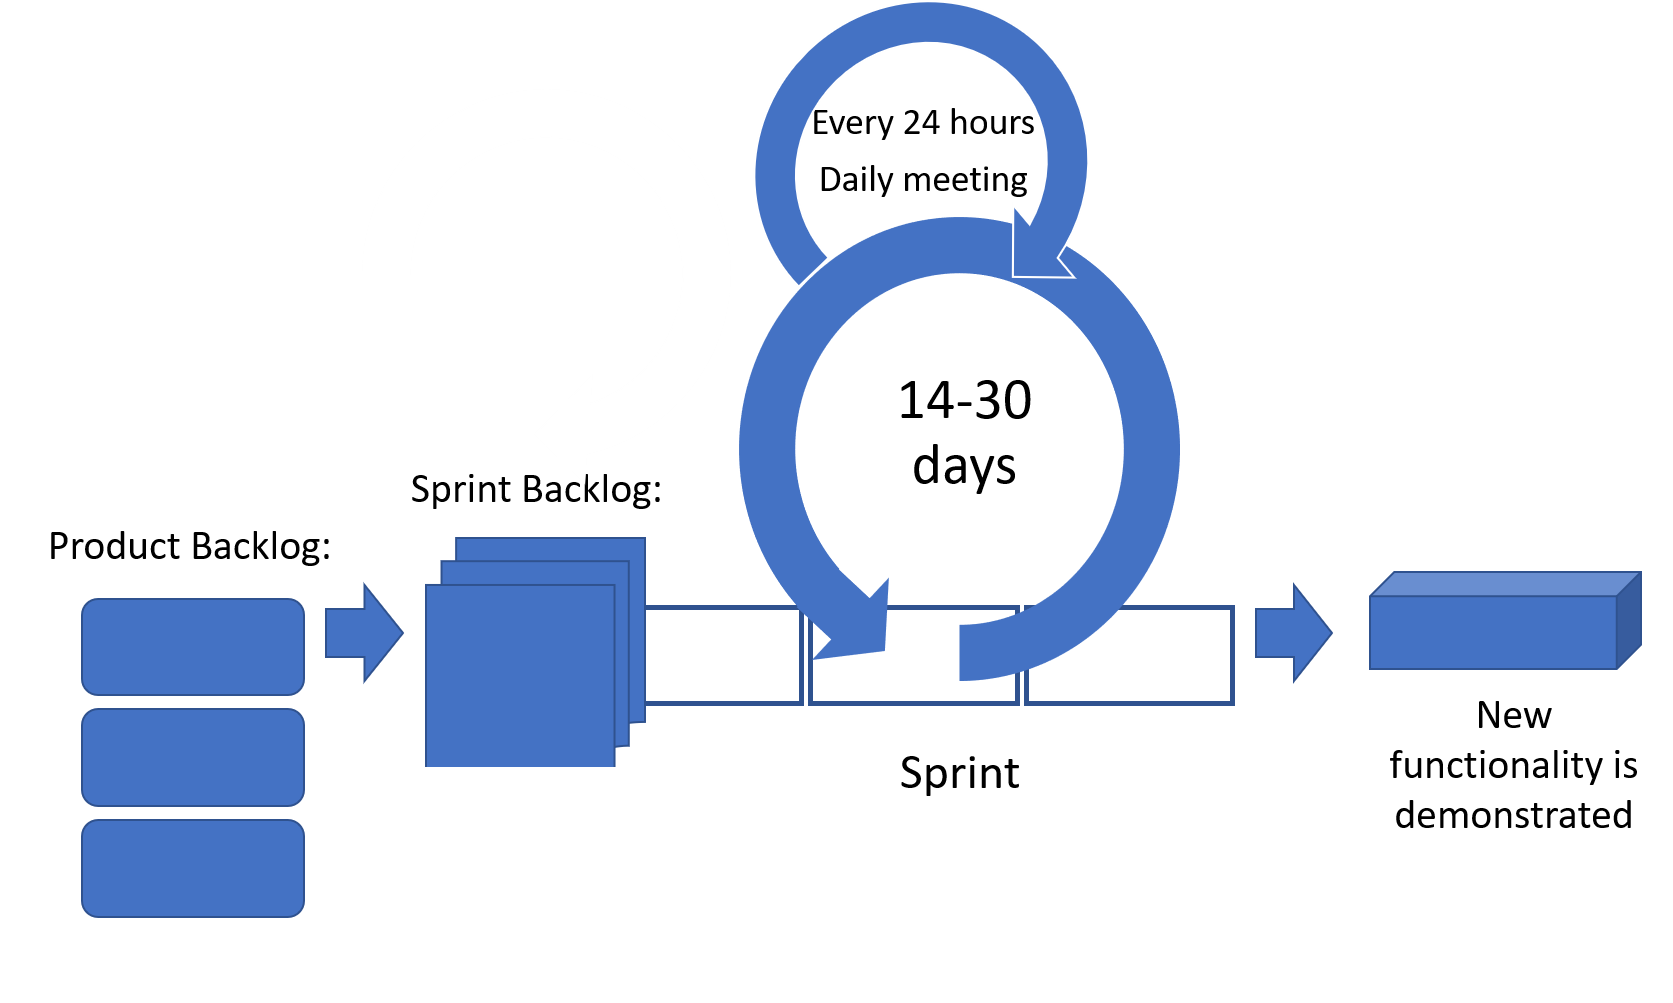
\includegraphics[width=.45\textwidth]{Figures/scrum.png}\quad

%\caption{The Scrum Methodology Life Cycle \cite{cohen2003agile}}
%\label{fig:scrum lifecycle}
%\end{figure}

%A User Story (US) describes functionality that will be valuable to the stakeholders. The most commonly used template for specifying USs is: ``As a <type of user>, I want <goal or objective>, [so that <some reason>]'' \cite{cohn2004user}. For example: "As a Manager, I want to review content before it is published so that I can assure it is appropriate".
%Each US describes what the desired functionality is, who uses it for, and may include also the reason why it is useful.
%USs are usually complemented with conversations and tests.
%Besides using the template for specifying USs, they can be defined as a feature representation that customers want in the product \cite{kassab2015changing}, or as operational documents that describes user functionalities on a low-level basis \cite{wautelet2014unifying}. There are various definitions and specifications to US, where they all rely on the foundation defined in \cite{cohn2004user}.
%However, in the bottom line, all the definitions and specifications rely on Mike Cohn \cite{cohn2004user} definition.  %[Yuval] did we say anything about this definition? 

%USs work well with iterative development. They start with an epic, which is supposed to be a large scale task or feature, %for example - a task of "Home page refactor",
 %that can not be delivered as defined within a single iteration.
%which is defined as a large US that can not be delivered as defined within a single iteration. Then, the epic is split to smaller user stories which fit the iterative work. 
%then, the epic is split into to smaller tasks/USs which fit the iterative work. 
%The product owner prioritizes the stories and in the sprint planning meeting the team identifies the stories they are committed to during the sprint. Furthermore, USs encourage continuous conversations between developers and users, facilitating rapid feedback cycles \cite{cohn2004user}, which leads to increased understanding.

%Managing USs is challenging and thus various platforms were developed to support this task. One of the common platforms for the purpose is Jira. %\footnote{\url{http://www.atlassian.com/software/jira/}}. 
%Jira is a project and issue tracking product that fits in agile project management that consists of issues management, sprints planning, tasks distributing across the software team, and tracking the issues. It further supports the management of the activities history. 
%The Jira tool is widely used for issue tracking in software development projects, especially ones who work in Agile methodologies \cite{ortu2015jira}.


%Given the popularity and the wealth of information that Jira holds, we decide to extract data from projects that work with Jira Scrum method. In Jira, the project requirements are written as issues, which are the building blocks of any Jira project. An issue could represent a US, a bug, a task, or another issue type. In this work, we refer to USs and similar types- new features and sub-tasks which we call them User Stories Issues (USI), and omit bugs, epics, and tasks.

%[Arnon - need to refer to paper "Rapid quality assurance with Requirements Smells". Also, there is a need to look for studies related to issues quality. In addition, for ML related studies, mention the goals, the algo used, the dataset, the features, and the results, this would enable us to better analyze the existing studies and explicate the gaps]
% Yarden - I added the paper "Rapid quality assurance with Requirements Smells" although I'm not sure it is relevant. The ML studies mentions in the sub section Data-Driven Evaluation of User Stories, I wrote about their methods, I don't think there is a need to specify about every detail since it will be very long. I looked for studies related to issues quality and all I entered here all I found.  


\section{Related Work}
\label{sec-relatedwork}
When referring to user stories (US) evaluation, there are two main directions that are being studied: (1) Evaluation of the US quality; and
(2) Estimation of development efforts; 
%and (3) Data-driven evaluation of USs. 

%Other two directions relate to (4) Requirement analysis and classification (which relates to different formats of software requirements); and (5) Other evaluations of USs.
%There is an additional direction that relates to the field of US study indirectly. It relates to the analysis and classification of different formats of specification software requirements besides the US. 

%In this section we will review all the directions that have been studied in the US field, and present the contribution of our research and its difference from the existing works in the field.

%\subsection{Evaluation of USs}
%Many studies relate to the evaluation of USs, aims to support the developers and improve the development process. Common evaluation of USs is quality, where other evaluations relates  
\subsection{Evaluation  of User Stories Quality}


% Another similar research also refers to quality, but instead of talking on the US quality, it relates to requirements quality \cite{femmer2017rapid}. They called it requirements ``smells'' (bad), as code ``smells'' but for requirements. In this work, they  use requirements language criteria to derive the
% smells which they defined. \roni{What is a ``requirement language criteria''??}
% They create an automatic system that find violations in the requirements, based on the language annotations, and present the 
% findings and the summary of the results. 
% %smells


%In this section, we review the main works that relate to US quality evaluation.
%Studies on USs quality evaluation suggest quality criteria for such evaluation.

According to Leffingwell~\cite{leffingwell2010agileINVEST}, a US needs to capture the essential elements of a requirement: who used it for, what the desired functionality is, and why it is important. In addition, Leffingwell defined a set of criteria for evaluating US, such as independent, negotiable, valuable to users or customers, estimable, small and testable (INVEST) \cite{leffingwell2010agileINVEST}. This approach is very broad and serves as a basis to some other quality models which extend and add measures to these six criteria.

%There are several main works relates to USs quality, which most of them suggest quality criteria for USs quality evaluation, each defines other US quality criteria.

%Lai \cite{lai2017user} proposes a model for US quality measurement to reduce the risks of requirement changes in agile software development. 
Lai \cite{lai2017user} defined three factors for evaluating US quality: Basic Quality (Discussable \& Estimable), Management Quality (Controllable \& Manageable) and Acceptance Quality (Confirmable). Each factor consists of three metrics, with different weight, and the final quality metric is the weighted sum of all the three factors. 
They also suggested rules for correcting low-quality US. 
%By the acceptance criterion, it decides if there is a need for increasing the US quality and suggests rules for correction. [[RONI: What is this acceptance criteria? not clear]]

Lucassen et al. \cite{lucassen2015forging} presented the Quality User Story (QUS) framework, which is a collection of 14 criteria that determine the quality of USs. 
%in terms of syntax, pragmatics, and semantics. 
Using this framework, they developed an automatic tool called AQUSA \cite{lucassen2016improving}, which uses NLP techniques to detect US quality defects.
Each quality criteria is classified according to three concepts from linguistics: syntactic, semantic, and pragmatic. 
%In addition to these criteria, there is a need to check that each US consists of one role, one means, optionally one or more ends, and some pre-defined template as agreed upon among the stakeholders. [[Roni: vague sentence - what does it mean??]
Femmer et al.~\cite{femmer2017rapid} defined a set of ``requirements smells'', which are
undersirable requirement properties and created an automatic system called Smella to detect requirement smells. 



% The studies we discussed so far 
All the above studies analyze and classify requirements by defining rules over the textual description of the requirement or by following expert classification. 
The limitation of this approach is that often there is no empirical evidence that establishes the correctness of the defined rules, and they are given as axioms. 
For example, many studies recommend that user studies follow the following template ``As a $<$type of user$>$, I want $<$goal or objective$>$, [so that $<$some reason$>$.'' 
However, to the best of our knowledge, there is no empirical evidence that indicate that a US that follows the standard template is more likely to be understood by the developers.
% define a US quality criteria rely on this template. 
% it is often regarded as a best practice to use the following template 
% the most 
% of user stories is the one presented in \cite{lucassen2016use}: ``As a $<$type of user$>$, I want $<$goal or objective$>$, [so that $<$some reason$>$'', and many studies that define quality criteria rely on this template. However, %from the analysis of available data we derived from several real-world projects,
% we notice that this template is not always
% used. Moreover, to the best of our knowledge, there is no empirical evidence that indicate that a US that follows the standard template is more likely to be understood by the developers.
% These important studies indicate quality factors of USs and further emphasize the essential parts they should include. \roni{too vauge and unclear}
% In this work, we take a complementing approach in which we evaluate a US by measuring the development process of implementing it. 



% impact it of these qualities on the development process and the extent to which these these qualities are important to follow.



%One of the most important parts using US in the development process is that when a
%developer starts working on a US, he understands what to do and can %correctly implement it.
%The template and other quality criteria defined in previous studies in Section \ref{sec-relatedwork}, do not necessarily provide a satisfying assessment about the US understanding, and it's quality in the aspect of the development process. A US that contains the template and stands with the quality criteria, may still be misunderstood by the developers, or the
%other way around, it may be perfectly understood though it does not follow some of the quality criteria.





%While they covered the theoretical aspect, our work will focus on a measure that testifies on the US quality in the context of the work process and retrospect metrics.

\subsection{Effort Estimation in Software Development}

% When developing a software project, the time and punctuality are very important, as each delay may increase the cost and may result in unsatisfied customer. Therefore, a reliable estimation of development efforts allows scheduling the work-log with fewer mistakes and delays, in addition to providing a correct time assessment to the customer.
% One of the common fields in studies that relates to US are 

Effort estimation is the task of estimating the development efforts of implementing a given requirement. This topic has been widely studied for many years. 
In the context of US effort estimation, non-automated methods for effort estimation such as planning poker have been proposed and used in practice~\cite{mahnivc2012using,haugen2006empirical}.
A variety of automated methods have been proposed for US effort estimation~\cite{ziauddin2012effort}, including methods based on Deep Learning~\cite{choetkiertikul2018deep,porru2016estimating,abrahamsson2011predicting} and 
Dynamic Bayesian Networks \cite{hearty2008predicting}. 
The data used by these methods is extracted from the US text. 

% Story point estimation
The effort of implementing a user story is often measured in \emph{story points} as oppose to actual time. 
A story point is a \emph{relative} unit of measure that is used by the development team ``to provide relative estimates of effort for completing requirements'' it~\cite{story_point_definition}. 
Choetkiertikul et al.~\cite{choetkiertikul2018deep} proposed a data-driven method to estimate the number of story points assigned to a US, using a deep learning method that contains an LSTM layer and a recurrent highway net.

% User stories are often
% In the context of effort estimation, \cite{choetkiertikul2018deep} tries to predict the story points of an issue. In particular, it predicts the story points by analyzing the text. For the classification task, it builds a model using deep learning, which contains LSTM layer, recurrent highway net, and in the end, the regression that predicts the story points.

% and 
% Many studies aim to evaluate or predict the development efforts of implementing a US. 
% Some of these attempt at predicting efforts using machine learning and deep learning approaches relaying on data extracted from the US text  \cite{choetkiertikul2018deep,porru2016estimating,abrahamsson2011predicting}. 
% Others propose an effort estimation algorithm based on other methods such as dynamic bayesian networks \cite{hearty2008predicting} or develop models that evaluate the implementation effort by ranking USs criteria, such as complexity, see for example the work of Ziauddin et al. \cite{ziauddin2012effort}.
% Others studies refer to how  developers estimate the efforts, and relies on expert opinions such as the planning poker technique \cite{mahnivc2012using,haugen2006empirical}. 

The objective of all effort estimation methods is to be as accurate as possible. 
This is a different task from the one this paper addresses, which is to evaluate the quality of US -- a US that requires significant effort to implement is not necessarily a poorly written US. 


In another study, Choetkiertikul et al.~\cite{choetkiertikul2017predicting} aimed to predict delays experienced when implementing USs. 
In their prediction model, they used text-based topic models, number of comments, number of effect versions, and additional process based information from \jira. It also compares different prediction times of the development process and uses several machine learning classifiers. 
% - Random Forests, Neural Networks, Decision Tree, Naive Bayes, NBTree, Deep Neural Networks with Dropouts, and Gradient Boosting Machines 
This work is reminiscent to our impact-driven approach. However, note that implementation delays may result from a variety of reasons that are not related to US quality, such as an incorrect effort estimation or the complex of the requested functionality. 
% from the existing studies is that we focus on the assessment of the USs in context of the text, during the development process so to improve the understanding of the developers and to reduce inaccurate implementations. \roni{not clear} The second study, for example, focuses on issues that cause delays \cite{choetkiertikul2017predicting}. However, the delay might result due to other reasons than the US quality, such as an incorrect estimation of the time or a complex request.



% a US it does not mean the US was of low quality.  
% Yet, these studies neglect the quality of the US. It is possible that the USs being estimated are poorly
% written, and thus may affect the estimation. Thus, there is a need to first check and improve the quality of USs. 

% \roni{I don't see the point of this subsection. The effort estimation above is also data driven.}
% \subsection{Data-Driven Evaluation of User Stories}

% An emerging research area for evaluating USs refers to data analysis. Various studies deal with extracting issues from open source projects and predicting some information on the issues that affect the software development process.






%What distinguish our work from the existing studies is that we focus on the assessment of the USIs in context of the text, to improve the understanding of the developers and to reduce wrong implementation. In the presented study \cite{choetkiertikul2017predicting}, for example, the study focus on issue that will cause delays. However, the delay might result due to other reasons such as wrong assessment of the time or a complex request. 

% According to our goal, we develop a model and extract the desired features. 


%[Arnon] need to check how it fits in. Yarden, maybe we don't have to add it. If we do want to add this, we need to add a different subsection as it written now.
%\subsection{Requirements Analysis and Classification}

%As explained in the previous section, a US is a common format to describe requirements, which are one of the main parts in the software development process. Besides USs, other studies analyze and classify other types of software requirements, for example, feature requests from the "SourceForge"\footnote{\url{https://sourceforge.net/projects/issue-tracker/}} issue tracker. %different types of Jira issues or other issue trackers. 
%A common classification of the requirements in those studies is the classification of a text of whether it represents a requirement or not \cite{choetkiertikul2017predicting,choetkiertikul2018deep,dollmann2016and}. Other studies also add classification of semantic annotation. The latter classification is facilitated by using natural language processing tools \cite{vlas2011rule}, and machine learning approaches \cite{dollmann2016and}. These studies aim to improve the requirements, the life-cycle understanding and the project scope understanding, so to improve software development. For that purpose, they developed tools that classify and analyze the requirements in the context of semantic annotation, and compared their results to expert and manually classification. These works are similar to ours in the idea of classifying requirements to improve software development. But the classification definition is different, and while they use experts tagging, we are using impact-driven approach, that is, checking the implications on the development process.
%While their results compared to expert and manually classification. 


%We presented three aspect relate to user story research, how they contribute to the use in USs and improve the work with them in different ways. Each of them contribute to the development process in different way. While the first aspect relates to the quality of US, the second relates to the estimation of development efforts, and the last contribute to the development process by data-driven evaluation of USs. What distinguish our work is that we are looking on the impact of the user story on the development process and guide by it. We aim to support the development process and to alert on US that need to re-write and prevent changes and delays during the sprint.

\section{The Stability Metric}
\label{sec-impactmetric}
%Here we propose several metrics for assessing USI. 
%Then, we say we focus on the changes since it is in the sprint. 
%Defining that one and calling it a \emph{stable} USI.



%As mentioned before, while using US in software development is very common, only a limited attention has been paid to assess their actual quality in terms of their readiness for implementation. In this section, we first analyze the limitations of current approaches for assessing USs. Next, we introduce a new set of data-driven metrics. Next, we introduce the data we used, run these metrics on USs collected from several real-world software projects and present statistics about them. Finally, we focus on a specific, novel, metric to assess US that we call stability.


%\subsection{Limitation of Current Quality Metrics}

% For assessing user stories, the first challenge is to find the proper metrics, in particular, in the context of the development process. 
% We aim at a situation in which a US will be understood and ready for implementation, so it will not cause problems and delays during the development process. For that purpose, we seek for metrics for evaluating US focusing on the potential impact on the development process. 
% By identifying USs that may be misunderstood, it is advisable that these should be fixed so to decrease the misunderstanding of the developers and save their resources. \roni{All this was said before already twice, one time in the introduction and one time int he background and related work section}



%\subsection{Measuring the Impact of User Stories}

% High-level idea
In this work, we propose a novel type of US metrics, aimed to capture the following rationale.  
The main objective of writing a US is to concisely communicate some requirement. % to enable its implementation. 
% \emph{before and during the time} in which it is implemented. %, and the main objective . 
%A poorly written US is therefore a US that poorly communicates the requirement prior to and during its implementation. 
Poorly communicating a requirement is expected to make its implementation more difficult and have other negative effects on the development process. 
Therefore, we propose to evaluate a US in retrospect by analyzing that development process in which it is implemented, as oppose (or in addition) to  analyzing the text in the US that describes it. 
We refer to metrics that evaluate user stories in this way as \emph{impact-driven} US metrics. 
% the US metrics we propose 
% Thus, the impact-driven US metrics we describe below assess the quality of a US by analyzing that development process in which it is implemented, as oppose to analyzing the text in the US that describes it. 
\roni{IMPORTANT: READ THIS CAREFULLY AND COMMENT EDIT!!!}
%a US, impact-driven US metrics assess a US by analyzing the development process that implemented it. 



% low-quality USs should 
% Thus, the main success criteria for a US should be related to 
% if a US fails to do so, i.e., fail to communicate the requirement when it is implemented, then its quality is low. 


% In particular, we propose metrics that aim to (indirectly) estimate if a US is properly understood and sufficiently detailed so that it can be implemented. 



% a US that is poorly written will not be properly understood and consequently be more difficult to implement and have negative effects on the development process. 


\subsection{Using User Stories in \jira and Scrum}
The impact-driven metrics we propose are described in the context of the \jira issue tracking tool and the popular \emph{Scrum} software development methodology~\cite{schwaber2002agile}. 
% Some background on SCRUM
Software development in Scrum progresses through \emph{sprints}, where every sprint is a ``time-box of one month or less during which a ``Done'', usable, and potentially releasable product increment is created''\cite{schwaber2017agile}. 
A \emph{product increment} in Scrum is a set of \emph{backlog items}, where every backlog item in Scrum represents a development task, e.g., implementing a user story or fixing a bug. 
The \emph{product backlog} is a list of all backlog items that are of interest. 
Throughout the development process, backlog items are updated, added and deleted from \emph{product backlog}. 
At the beginning of each sprint, a set of issues are added to the \emph{sprint backlog}, with the intention of finishing implementing them during the sprint. 
The duration of a sprint is fixed throughout the project, and a new sprint starts immediately after one finishes. 


% Scrum in \jira, introducing USI
Scrum is commonly implemented in the \jira issue tracking system. 
Every backlog item in Scrum corresponds to a \emph{\jira issue}. 
\jira allows associating types to issues, e.g., ``Bug'' and ``User Story''. 
This research focuses on issues of the latter types, referred to as User Story Issues (USIs). % in Jira is ``the smallest unit of work that needs to be done.''\footnote{https://confluence.atlassian.com/adminjiracloud/issue-types-844500742.html}





% Thus, while like all Agile methodologies Scrum is designed to ``embrace change''~\cite{fowler2001agile}, Scrum strictly discourages changes to a USI after it is assigned to a sprint and a developer to be implement.  
% The core of the impact-driven metrics we consider is to measure changes done to a USI \emph{after} it is assigned to a sprint backlog.

\subsection{Impact-Driven Metrics}
\jira manages and stores an abundance of information about every USI, including when it was created, when it was added to a sprint, who wrote it, and its current status (e.g., implementation has not started, in progress, and completed). 
In particular, \jira tracks all the changes performed on every USI, marking when they occurred and what was changed. 
Based on this information, we propose and discuss several potential impact-driven USI metrics. 


% MS metric
\subsubsection{Time to Completion}
According to Scrum best practices, a USI should be a short requirement that can be completed during a single sprint. 
Thus, if implementing a USI requires more than one sprint, this could indicate that the requirement was too long, included too much functionality, or was badly written. 

To quantify this observation, we consider the following impact-driven metric. 
Let $x$ be a USI we want to evaluate, and let $\sprints(x)$ denote the set of sprints that $x$ was assigned to. 
That is, $\sprints(x)$ is the set of sprints in which $x$ was added to their sprint backlog, until the status of $x$ has changed to ``Done''. 
%\roni{What about USI that were removed or marked as ``duplicate'' or ``cancelled''?}
The first impact-driven metric we propose is $|\sprints(x)|$, which estimates \emph{the number of sprints required to implement a USI}. 
This metric is can be extracted automatically from \jira. 
%by summing the number of sprints which included a USI until its status has changed to ``Done''.  

The problem with this metric is that there are other, common, reasons for why multiple sprints are needed to implement a USI. 
For example, a delay in the implementation of a higher priority USI assigned to the same sprint may cause the implementation of our USI to also be delayed and ``drag'' to the subsequent sprint. 
While this is not desirable, it does not indicate that our specific USI has been poorly written. 

\subsubsection{Changes During a Sprint}
Like all Agile methodologies, Scrum is designed to ``embrace change''~\cite{fowler2001agile}. 
However, Scrum strictly discourages changes to a USI after it is assigned to a sprint and a developer to be implement. 
That is, while a USI is in the product backlog, the team should discuss it and change its description and other properties. However, a USI should enter a sprint backlog only after the team discussed it and agreed that it is sufficiently defined, and ready to be implemented~\cite{buglione2013improving}. 
Based on this, we propose two impact-driven metrics that measure changes made to a USI after it has been assigned to a sprint. 
% The first measures changes in effort estimation, and the second measures changes
% and the sprint has begun. 


\paragraph{Changes to the effort estimation.}
This metric consider changes in effort estimation, namely, changes made to the number of story points assigned to a USI. 
Such a change during a sprint may indicate incorrect interpretation of the US, suggesting that the USI is poorly written. 


% and hence lead to a wrong effort estimation.
The main limitation of this metric is similar to that of the number of sprints metric: there are other, common, reasons for why the number of story points may change during a sprint. 
Accurate effort estimation in software is notoriously difficult, and thus changes to story point may be due to incorrect estimation of the technical difficulty of implementing a task as oppose to lacking description of the requirement. 
Also, the developer that made the effort estimation for USI $x$ may be more experienced than the developer that is assigned to implement $x$, and thus under-estiamte the effort required to complete $x$. 
So changes to the number of story points do not necessarily indicate that the quality of the USI  is low. 


\paragraph{Changes to the textual description.}
This metric measures changes to the textual description of the USI done after it has been assigned to a sprint. 
% Indeed, we do not expect to see changes and edits in a USI description after the sprint starts since at this stage the focus should be on implementation. 
Change in the textual description of a USI implies that it was not well defined, misunderstood, includes ambiguities, or lacks of details. 
This does not mean that changes do not occur during implementation. 
However, since US are rarely used for documentation purposes, the fact that a developer took the time to update a US during a sprint suggest that this change is required now to implement it. 
We call this metric \emph{USI Stability}. 
\begin{definition}[Stability] 
The stability of USI $x$ with respect to sprint $y$, denoted $\stability(x,y)$ is the number of words in the textual description $x$ that have changed after $x$ was assigned to $y$. 
A USI $x$ is $\epsilon$-stable if total stability with respect to all sprints it was part of is at most $\epsilon$. 
That is, $x$ is $\epsilon$-stable iff 
\begin{equation}
    \sum_{y\in\sprints(x)}\stability(x,y)\leq \epsilon
\end{equation} 
\label{def:stability}
\end{definition}
% Note that an $\epsilon$-stable USI posses the property that it if its stability with respect to the first sprint that included $x$ in its sprint backlog is at most $\epsilon$. 
A USI is said to be $\epsilon$-unstable if it is not $\epsilon$-stable. 
We observed that it is often the case that the textual description of a USI is modified immediately after it has been added to a sprint. Such changes are most likely the result of discussions made just before adding the USI to the sprint. Thus, when computing the stability of a USI, we ignored changes made in the first hour after it has been added to the sprint. 

% it introduces with certain changes before it moves into implementation, this is actually a desired practice and we would not like to consider it as a change. Thus, in this work, we allow for 1 hour delay after the USI enters a sprint, before checking the changes. \roni{Too vague. WHy is it desired?}



% \begin{equation}
%     x \textit{ is } \epsilon \textit{-stable iff} \max_{s\in\sprints(x)}\leq \epsilon
% \end{equation}
% We ignored all changes made in the first hour after the USI is assigned to a sprint, assuming these changes are still considered part of the sprint planning stage. 




%as we associated theseobserved these changes are
% is the number of words that have been changed since the sprint has started.

% called \emph{$\epsilon$-stable} if the number of changes made to it after it entered a sprint is at most $\epsilon$. 
% A USI that has more changes after it enters a sprint is called \emph{$\epsilon$-unstable}.


% \begin{definition}[$\epsilon$-Stablity]: a USI is called \emph{$\epsilon$-stable} if the number of changes made to it after it entered a sprint is at most $\epsilon$. 
% A USI that has more changes after it enters a sprint is called \emph{$\epsilon$-unstable}.
% \end{definition} 

% To determine stability, there is a need to set a threshold for the number of words that have been changed. 

\subsection{USI Stability in the Wild}

Since stability is a novel metric for USIs, we examine below its values in USIs from real-world projects. 

\subsubsection{Data Collection}


\begin{table}[h]
    \centering
    \begin{tabular}{l|r|r|r|c}
	 \toprule
    %\cmidrule(rl){1-4}
    Project & Created & Issues & Sprints & Avg. Words \\
    \midrule
    %\cmidrule(rl){1-1}\cmidrule(rl){2-2}
      Alfresco (REPO)
      & 2015
      & 2,457
      & 138
      & 64    \\
      JBossDeveloper (DEVELOPER)
      & 2015
      & 5,379
      & 129
      & 55    \\
      LSST (DM)
      & 2014
      & 20,106
      & 276
      & 48    \\
      Spring (XD)
      & 2013
      & 3,710
      & 66
      & 40    \\
    %   Commercial                    
    %   & n/a
    %   & n/a
    %   & n/a
    %   & n/a   \\ 
      \bottomrule
    \end{tabular}
    \caption{General statistics from the open-source projects in our dataset.}
\label{tab:statistics}
\end{table}


We collected USIs from the following open-source projects. 
\begin{itemize}
	\item \textbf{Alfresco (REPO).}\footnote{\url{https://issues.alfresco.com/jira}} 
	An enterprise-class, cloud-native content services platform. 
	\item \textbf{JBossDeveloper (DEVELOPER).}\footnote{\url{https://issues.jboss.org}} 
	A developer environment that integrates with the JBoss application server.
	\item \textbf{LSST (DM).}\footnote{\url{https://jira.lsstcorp.org}} Software services 
	for a vast astronomical dataset.
% 	and systems for LSST's data products. %to build a well-understood system that provides a vast astronomical dataset for unprecedented discovery of the deep and dynamic universe.)
	\item \textbf{Spring (XD).}\footnote{\url{https://jira.spring.io}} 
	An application framework and inversion of control container for the Java platform.
	\item \textbf{Commercial.} A software project in a large multinational corporation that specializes in software and services.
	%need to add meta data
\end{itemize}
In addition, we collected USIs from a software project in a large multinational corporation that specializes in software and services.
Thus, our dataset comprised USIs from four open-source projects and one commercial project. 




%and consists of four open-source projects and one commercial projects. 
% projects, and different subjects which will detail next.
% Description of the projects
% The data collected in this research originated from projects that manage their software development process with the Jira issue tracking software. %[Arnon - need to better justify the selection of the projects, maybe elaborate on the criteria and the quest for such projects]. Yarden- I add.
% We searched for projects that follows the Scrum methodology, which work with sprints and user stories. 
%They were randomly chosen and contain different size of projects, and different subjects which will detail next.

% We collected from these projects all USIs that were closed and were part of a sprint, so the work on these issues was over and the entire history changes was also available.
%[Arnon, maybe add more meta-data for each project - duration (when its starts), number of classes, number of developers, etc..] Yarden- I add.
% The open sources projects we used in this study were the following:
% \begin{itemize}
% 	\item \textbf{Alfresco- REPO}\footnote{\url{https://issues.alfresco.com/jira}} - enterprise-class, cloud-native platform that enables organizations to build digital operations to deliver instant services with exceptional experiences. 
% 	(The project started on 2015 and includes 2,457 issues and 138 sprints)
% 	\item \textbf{JBossDeveloper- DEVELOPER}\footnote{\url{https://issues.jboss.org}} - provides the tools, technologies, and community to building and delivering modern, innovative apps and services.
% 	(The project started on 2015 and includes 5,379 issues and 129 sprints)
% 	\item \textbf{lsst-DM}\footnote{\url{https://jira.lsstcorp.org}} - creating the software, services and systems which will be used to produce LSST's data products. %to build a well-understood system that provides a vast astronomical dataset for unprecedented discovery of the deep and dynamic universe.)
% 	(The project started on 2014 and includes 20,106 issues and 276 sprints)
% 	\item \textbf{Spring-XD}\footnote{\url{https://jira.spring.io}}- solving common big data problems such as data ingestion and export, real-time analytics, and batch workflow orchestration. %XD stands for "eXtreme Data"
% 	(The project started on 2013 and includes 3,710 issues and 66 sprints)
% 	\item \textbf{Commercial company}- A multinational corporation that specializes in software and services.
% 	%need to add meta data
% \end{itemize}

From each project, we only collected USIs have been completely implemented (i.e., marked as \emph{closed}) and have been included in a sprint. 
These two conditions are needed to be able to compute stability. 
Table~\ref{tab:statistics} present descriptive statistics about the data we collected from the open source projects. 
Specifically, Table~\ref{tab:statistics} lists when each project was created (the ``Created'' column), the number of Jira issues in these projects (``Issues''), 
the number of sprints in which these USIs were in (``Sprint''), 
and the average number of words in each USI (``Avg. Words''), ignoring stop words. 


In our analysis below, we considered $\epsilon$ values of 5 and 20 when checking for $\epsilon$-stability. These values where chosen to represent a small change (5 words) and large change (20) in the USI. Note that the average number of words per USI in all projects is between 40 to 64 (see Table~\ref{tab:statistics}), and thus 5 and 20 changed words correspond to a change in approximately 10\% and 40\% of the words in a USI. 





% Description of the results

\subsubsection{Results}

% label statistics ratio
\begin{table}[h]
    \centering

    \begin{tabulary}{\textwidth}{lccc}
    \toprule
    %\cmidrule(rl){1-4}
    Project & \hfil USI & 5-\emph{unstable} & \hfil 20-\emph{unstable}\\
    %\midrule
    \cmidrule(rl){1-1}\cmidrule(rl){2-2}\cmidrule(rl){3-3}\cmidrule(rl){4-4}
      Commercial  & 1855 & 377 (20\%) & 235 (13\%) \\ 
      DEVELOPER   & 1229 & 394 (32\%) & 290 (24\%) \\
      REPO        & \phantom{0}900  & 195 (22\%) & 140 (16\%) \\
      XD          & 1741 & 173 (10\%) & 80 (5\%) \\
      DM          & 4962 & 626 (13\%) & 415 (8\%) \\
      \bottomrule
    \end{tabulary}
    \caption{List of the number of the two types of \emph{unstable} USI-
    changes in more than 5 words and changes in more than 20 words, in all the different projects (in brackets the percentage of these from all the USIs)}
\label{Table:lable ratio}
\end{table}

% First, we check the ratio between \emph{stable} and \emph{unstable} USIs in each one of the projects. 
Table \ref{Table:lable ratio} shows the number (and percentage) of 5-unstable and 20-unstable USIs in all projects. 
%The rows represents the different projects, the second column represents the number of USIs in each project, the third column represents the number of \emph{unstable} USIs by the label of change in more than five words (and the brackets represent the percentage of these), and the last column represents the same, for the second label - change in more than twenty words.
The results show that most USIs are 5- and 20-stable. 
For example, in the XD project there are 1,741 5-stable USIs and only 80 USIs are 20-unstable. 
Having more stable USIs than unstable supports our rationale that making changes to a USI during a sprint is not desirable. 
Also, we do not see significant difference between the commercial and open-source project. 


% This supports our makes a perfect sense, because a change means instability, so we do not expect to see a lot of it. Referring to the open source projects, it is interesting to notice that the smaller projects have a higher ratio of \emph{unstable} USIs then the large projects. When comparing the commercial project to the open source projects, it seems that they have similar characteristics. 


Next, we considered \emph{when} the changes that comprise the stability value occur during a sprint. 
% That is, when most changes occur and the behavior of the changes during the sprint.
% how the
% We were also interested in examining the number of changes along the time after entering a sprint. 
% This information can help us understand the work process, when most changes occur and the behavior of the changes during the sprint. 
Figure \ref{fig:changes after sprint} presents the average number of changes in a USI in the first two weeks after the USIs enter the sprint, for all projects in our dataset. 
It is evident that most of the changes happen in the first day of the sprint for all the projects, and there are fewer changes as the sprint progress. 
These results are not surprising, as on the first day, the developers start working on the USIs that were added to the current sprint. Thus, if something is not clear, the higher probability it comes up during this time. 
Our goal is to lower the amount of changes during this time frame by predicting such unstable USIs, so developers are able to move into implementation as soon as possible. 

\begin{figure}[ht]
\centering
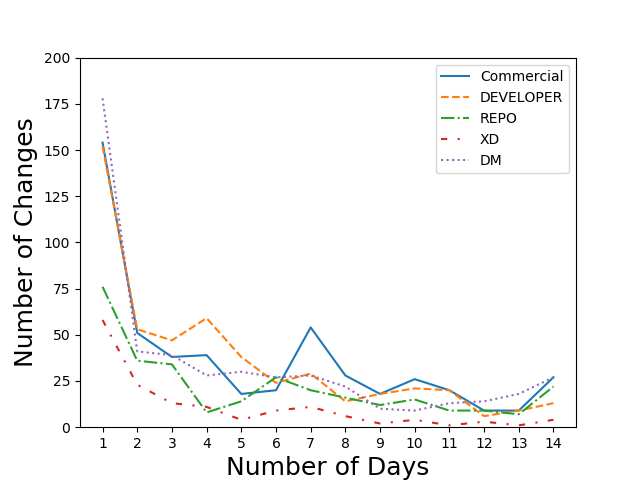
\includegraphics[width=.45\textwidth]{Figures/number_changes_after_sprint_two_weeks_only_new.png}\quad

\caption[Number changes two weeks]{\centering Number of changes after the sprint started in the first two weeks}
\label{fig:changes after sprint}
\end{figure}

\roni{up to here 31/7}

% This 
% It indicates that the data is imbalanced, for example, in the "XD" project there are 1741 USIs that are stable and only 80 USIs that are not. That is, most of the USIs are \emph{stable} and did not change during a sprint and the minority of the USIs are \emph{unstable} and were changed after they entered the sprint. This observation makes a perfect sense, because a change means instability, so we do not expect to see a lot of it. Referring to the open source projects, it is interesting to notice that the smaller projects have a higher ratio of \emph{unstable} USIs then the large projects. When comparing the commercial project to the open source projects, it seems that they have similar characteristics. 

%Having projects with different sizes, we are also able to check of whether the project size affect the resulting model.

%Another thing to notice from Table \ref{Table:lable ratio} is the different project sizes, from the small one - "REPO" with 900 USI to the large one - "DM"; In that way, we are able to examine our model on varied projects.

Next, we were interested to see if the USI stability is affected by the format for writing USI. \roni{Why are we interested in this?}Table \ref{Table:ratio template_5} presents the descriptive statistics for changes in at least five words, where the results of changes in at least twenty words is presented in Table \ref{Table:ratio template_20} and are similar to the results in \ref{Table:ratio template_5}. Overall, it seems that using templates have similar affect on changes when ignoring the use of a template. For that reason, we analyze all USIs together. 


\begin{table}[]
	\centering
	\caption{Ratio between change in the text and text written by template - 5 words}	
    \begin{tabular}{lccc}
	\toprule
	
	Project	& 
	\multicolumn{1}{p{1.5cm}}{\centering \% with template \\ } &
	\multicolumn{1}{p{1.9cm}}{\centering \% with template \\ \& with change } &
	\multicolumn{1}{p{1.9cm}}{\centering \% without template \\ \& with change } \\
	
	%Project	&
	%\% with template & \% with template and with change &  \% without template and with change \\
	\midrule
	Commercial & \phantom{0}4.4\% & 30.0\%           & 20.0\%  \\
	DEVELOPER  & \phantom{0}3.0\% & 24.0\%           & 32.0\%  \\
	REPO	   & 15.2\%           & 34.0\%           & 24.0\%  \\
	XD	       & 17.0\%           & 20.0\%   & \phantom{0}8.0\% \\
	DM	       & \phantom{0}0.1\% & \phantom{0}0.0\% & 13.0\%  \\
	% \hline
	\bottomrule
    \end{tabular}
    \label{Table:ratio template_5}
\end{table}



\begin{table}[]
	\centering
	\caption{Ratio between change in the text and text written by template - 20 words}	
    \begin{tabular}{lccc}
	\toprule
	
	Project	& 
	\multicolumn{1}{p{1.5cm}}{\centering \% with template \\ } &
	\multicolumn{1}{p{1.9cm}}{\centering \% with template \\ \& with change } &
	\multicolumn{1}{p{1.9cm}}{\centering \% without template \\ \& with change } \\
	
	%Project	&
	%\% with template & \% with template and with change &  \% without template and with change \\
	\midrule
	Commercial & \phantom{0}4.4\%  & 15.6\%           & 19.6\%  \\
	DEVELOPER  & \phantom{0}3.0\%  & 13.5\%           & 23.9\%  \\
	REPO	   & 15.2\%           & 24.8\%           & 13.8\%  \\
	XD	       & 17.0\%           & 11.4\%   & \phantom{0}3.1\% \\
	DM	       & \phantom{0}0.1\% & \phantom{0}0.0\% & 8.3\%  \\
	% \hline
	\bottomrule
    \end{tabular}
    \label{Table:ratio template_20}
\end{table}


% \subsubsection{Relation between USI template and USI stability}
% We were further 



% % ratio of stable and unstable in the test and train sets:
% % We are also interested to verify that 
% Next, we were interested to %verify that 
% examine if the ratio between \emph{stable} and \emph{unstable} USIs in both the train and the test set is similar. Table \ref{Table:train test ratio} presents this ratio for both of the thresholds we defined. It indicates that the ratio of \emph{unstable} USIs in the commercial project is lower in about 10\% in the test set compared to the train set, and this hold for "DEVELOPER" project as well. On the other hand, in the "XD" project, the situation is opposite. %, as we expected. 

% The different ratio between the train set and the test set affects the prediction task and makes it more challenging. 
% The classification algorithms used for the task at hand learn about the future from past experience, and since we have different patterns, i.e., different ratio in the train and test set in several projects, it may interfere with the learning. We wish to overcome this using the features we defined. 



% \begin{table}[]
%     \centering
%     \caption{List of the ratio of the two types of \emph{unstable} USI- 
%     changes in more than five words and changes in more than twenty words, in the train vs test set in all the different projects}
%     \begin{tabular}{l|c|c|c}
% 	 \toprule
%      \multicolumn{4}{c}{train} \\
%     \toprule
% 	Project & \hfil \# of USI & \# \emph{unstable} USI-5 & \hfil \# \emph{unstable} USI-20\\
% 	\hline
% 	Commercial  & 1483           & 335 (23\%)       & 217 (15\%) \\
%       DEVELOPER & \phantom{0}983 &  334 (34\%)      & 247 (25\%) \\
%       REPO      & \phantom{0}720 &  180 (25\%)      & 116 (16\%) \\
%       XD        & 1393           & 122 \phantom{0}(9\%) & \phantom{0}49 \phantom{0}(4\%) \\
%       DM        & 3970         & 509 (13\%) & 332 \phantom{0}(8\%) \\
% 	\toprule
%      \multicolumn{4}{c}{test} \\
%     \toprule
% 	Project & \hfil \# of USI & \# \emph{unstable} USI-5 & \hfil \# \emph{unstable} USI-20\\
% 	\hline
% 	  Commercial & 370 & \phantom{0}40 (11\%) & 17 \phantom{0}(5\%) \\ 
%       DEVELOPER  & 246 & \phantom{0}60 (24\%) &  43 (17\%) \\
%       REPO       & 180 & \phantom{0}48 (27\%) &  24 (13\%) \\ 
%       XD         & 348 & \phantom{0}51 (15\%) &  31 \phantom{0}(9\%) \\
%       DM         & 992 & 117 (12\%)           &  83 \phantom{0}(8\%) \\
%       \toprule
%     \end{tabular}
% \label{Table:train test ratio}
% \end{table}

%\begin{table*}[h]
 %   \centering
  %  \caption[train ratio]{List of the ratio of the two types of \emph{unstable} USI - changes in more than five words and changes in more than twenty words, in the train vs test set in all the different projects}
   % \begin{tabular}{c|c|c|c|c|c|c}
    %\toprule
	%Project & \hfil \# USI in train & \# USI in test & \# %\emph{unstable} USI-5 in train & \hfil \# \emph{unstable} USI-5 in test & 
	% \# \emph{unstable} USI-20 in train & \hfil \# \emph{unstable} USI-20 in test \\
%	\hline
	%Commercial & 1483 & 370 & 335 (23\%)& 40 (11\%) &  217 (15\%) &  17 (5\%)\\   
   %  DEVELOPER & 983 & 246 & 334 (34\%)&60 (24\%) & 247 (25\%)    & 43 (17\%)\\ 
    % REPO   & 720 & 180 & 180 (25\%)&48 (27\%) & 116 (16\%) & 24 (13\%) \\       
    % XD       & 1393 & 348 & 122 (9\%)&51 (15\%)& 49 (4\%)  & 31 (9\%)\\  
    % DM      & 3970 & 992  & 509 (13\%)& 117 (12\%)& 332 (8\%)&  83 (8\%)\\ 
     % \toprule
    %\end{tabular}
%\label{Table:train test ratio2}
%\end{table}

% We are also interested in examining the number of changes along the time after entering a sprint. 
%For that purpose, we first study when most of the changes happen, and second we study the ratio between \emph{stable} and \emph{unstable} USI throughout the development time.




% is assigned , one that measures effort estimation changes during a sprint, and one that measures changes to the textual description of the USI the number of changes to the stro
% The core of the impact-driven metrics we consider is to measure changes done to a USI \emph{after} it is assigned to a sprint backlog.


%     \item \textbf{Change in the story point after a USI assign to a sprint:} 
%     “A Story Point is a relative unit of measure, decided upon and used by individual Scrum teams, to provide relative estimates of effort for completing requirements“ \cite{story_point_definition}. 
%     Changes in the story point (SP) after the USI is assigned to a sprint may indicate incorrect interpretation of the text and hence lead to a wrong estimation.

% %%%%%%%


% Thus, a possible  MS impact-driven metric counts for  
%     and maybe it should have split into a few small requirements.  



% Multiple sprints metric relates to the number of sprints in which the USI was assigned to. 




% \begin{itemize}
%     % \item Missing text fields
%     \item \textbf{Multiple Sprints (MS):} A USI should be a short requirement that can be completed during a single sprint. Hence, if a USI lasts more than one sprint, this could indicate that the requirement was too long, included too much functionality, or was badly written. Thus, the MS impact-driven metric counts for  
%     and maybe it should have split into a few small requirements.  
%     \item \textbf{Change in the story point after a USI assign to a sprint:} “A Story Point is a relative unit of measure, decided upon and used by individual Scrum teams, to provide relative estimates of effort for completing requirements“ \cite{story_point_definition}. 
% %     Changes in the story point (SP) after the USI is assigned to a sprint may indicate incorrect interpretation of the text and hence lead to a wrong estimation.
%     \item \textbf{Change in the text after the USI is assigned to a sprint:} We do not expect to see changes and edits in the USIs after the sprint starts. Change in the USI text may imply that it was not well defined, misunderstood, includes ambiguities, or lacks of details.
% \end{itemize}

% The problem with the MS metric is that the multiple sprints do not necessarily point out a problem of the USI. It might be that the USI was hard to implement or there was a need to execute other urgent USIs instead, so it was postponed to next sprint. .

% The SP metric suffers from similar concerns as it may result from incorrect estimation of the development time or from different level of experience of the developers that results in different development time. So changes referring to SP do not necessarily relate to the quality of the USI and its understanding.





% one of which refer to the fact that a USI is assigned to a sprint only after it is well written and ready to execute \cite{buglione2013improving}. We propose data-driven USI metrics that measure the extent to which a given USI follows this ideal best practice. % In the following, we explain and discuss each of the metrics.
% The metrics we considered were the following:




% \jira manages and stores an abundance of information about every USI, including when it was created, when it was added to a sprint, who wrote it, and its current implementation status (e.g., implementation has not started, in progress, and completed). 


% , and backlog items that represent implementing a user story are k= 
% \jira and Scrum are commonly integrated, where USIs and other issues are created and moved to the sprint backlog as necessary. 



% The basic artifact in \jira is the \emph{issue}, which represent some development tasks. 




% %\subsection{Impact-Driven Metrics}
% % Following our observation that a user story template is used to a limited extent, we decided to refer to a more general term - user story issue (USI). \roni{No definition of USI??? what does it mean?? the reader will not know}Also not relevant here 

% \subsection{Impact-Driven Metrics}

% According to Agile and Scrum best practices, an ideal USI is one that should be concise and focused enough that it can be implemented in one sprint. 

% Before a USI is assigned to a sprint, the team may discuss and change it. 
% A USI should enter a sprint backlog after the team discussed it, and agreed that it sufficiently defined, and ready to be implemented. 

% Hence, we looked for best practices, one of which refer to the fact that a USI is assigned to a sprint only after it is well written and ready to execute \cite{buglione2013improving}. We propose data-driven USI metrics that measure the extent to which a given USI follows this ideal best practice. % In the following, we explain and discuss each of the metrics.
% The metrics we considered were the following: 

 
\section{Predicting User Stories Stability}
\label{sec-methodology}

For the task at hand, predicting user story stability, we utilize a Machine Learning (ML) techniques that automatically learn and improve from experience without being explicitly programmed. It is based on algorithms and statistical models that facilitate learning from existing examples about the future. ML techniques are divided into two main categories: \textit{supervised learning} and \textit{unsupervised learning}. 
%In supervised learning, the algorithms learn the past behavior using labeled examples in order to predict about the future behavior. 
Supervised learning approach are useful for predicting future behavior based on past behavior, in cases where information about the data and the expected outcome (label) are known.
% In unsupervised learning the data has no label, and it used to explore the data and discover hidden structures and connections. 
Unsupervised learning approaches are used for exploring the data, discovering hidden structures and patterns in the data, or separation to a number of groups where each group has similar properties, when there is no information about the the expected outcome.


In this study we use a supervised learning approach as we aim at developing a prediction model that is based on past experience with labeled data. Since we use USIs that were closed, we know if they were \emph{stable} or not. Thus, we have labelled data and can use supervised learning.


We adopt a common machine learning methodology that consists of the following steps: data collection, data preparation including data separation into train, validation and test sets, extraction of relevant features, and the optimization of hyper parameters.

\subsection{Data Collection}

The data collected in this research originated from projects that manage their software development process with the Jira issue tracking software. %[Arnon - need to better justify the selection of the projects, maybe elaborate on the criteria and the quest for such projects]. Yarden- I add.
We searched for projects that follows the Scrum methodology, which work with sprints and user stories. They were randomly chosen and contain different size of projects, and different subjects which will detail next.
We collected the data from four open sources software projects and one industry software project. We refer only to USIs that were closed and were part of a sprint, so the work on these issues was over and the entire history changes was also available.

%[Arnon, maybe add more meta-data for each project - duration (when its starts), number of classes, number of developers, etc..] Yarden- I add.
The open sources projects we used in this study were the following:
\begin{itemize}
	\item \textbf{Alfresco- REPO}\footnote{\url{https://issues.alfresco.com/jira}} - enterprise-class, cloud-native platform that enables organizations to build digital operations to deliver instant services with exceptional experiences. 
	(The project started on 2015 and includes 2,457 issues and 138 sprints)
	\item \textbf{JBossDeveloper- DEVELOPER}\footnote{\url{https://issues.jboss.org}} - provides the tools, technologies, and community to building and delivering modern, innovative apps and services.
	(The project started on 2015 and includes 5,379 issues and 129 sprints)
	\item \textbf{lsst-DM}\footnote{\url{https://jira.lsstcorp.org}} - creating the software, services and systems which will be used to produce LSST's data products. %to build a well-understood system that provides a vast astronomical dataset for unprecedented discovery of the deep and dynamic universe.)
	(The project started on 2014 and includes 20,106 issues and 276 sprints)
	\item \textbf{Spring-XD}\footnote{\url{https://jira.spring.io}}- solving common big data problems such as data ingestion and export, real-time analytics, and batch workflow orchestration. %XD stands for "eXtreme Data"
	(The project started on 2013 and includes 3,710 issues and 66 sprints)
	\item \textbf{Commercial company}- A multinational corporation that specializes in software and services.
	%need to add meta data
\end{itemize}



In the following we present descriptive statistics regarding the data set we worked with. Table \ref{Table:avg_word_num} presents the average number of words in USI for each project, ignoring stop words. We can notice that the values are between 40 to 64, where the average number of words in USI is 50.8. We wanted to examine small changes and large change, so we chose the threshold of 5 words to small change, which is about 10\% of the average number of words in USI, and 20 words to large change, which is about 40\% of the average number of words in USI. 

It might be that when a USI enters a sprint it introduces with certain changes before it moves into implementation, this is actually a desired practice and we would not like to consider it as a change. Thus, in this work, we allow for 1 hour delay after the USI enters a sprint, before checking the changes.



\begin{table}[h]
    \centering
    \caption{Average number of words in USI for all projects}
    \begin{tabular}{l|c}
	 \toprule
    %\cmidrule(rl){1-4}
    Project & \hfil Average number of words in USI \\
    \midrule
    %\cmidrule(rl){1-1}\cmidrule(rl){2-2}
      Commercial  & 47   \\ 
      DEVELOPER   & 55 \\
      REPO        & 64   \\
      XD          & 40  \\
      DM          & 48  \\
      \bottomrule
    \end{tabular}
\label{Table:avg_word_num}
\end{table}

%\section{Predicting User Stories Stability}
%\label{sec-methodology}
%Here will come the algorithmic part. 
%Explain how ML works very briefly, then what we did. 
%1) The high-level approach: mining the training set, extracting features.
%2) Explaining that we mine USI Repositories
%3) The feature families we used
%4) A word on the learning algorithm itself.

% In this section we will explain about the research methods and the stages of the process; In what tools we use, the features extraction, separation to train and test sets and the classifiers for the prediction task.

%To predict USI stability we adopt a machine learning approach. In the following, we briefly discuss the machine learning approach and then elaborate on the research methodology stages. 


%\subsection{Machine Learning Approach}
 

% In this study we use a supervised learning approach as we aim at developing a prediction model which predict base on past experience with labeled data. We use labeled USI with the stability indicator to predict the stability of new unlabeled USI. 


%%%%%%%%%%%%%%%%%%%%
%The research methodology contains the data collection, data preparation, the data separation into train, validation and test sets, the extraction of relevant features, and the optimization of hyper parameters.
%, and the evaluation of the results. 

%\subsubsection{Data Collection}
%The data was collected from projects that manage their software development process with the Jira issue tracking software. We collected the data from four open sources software projects and one commercial software project. We refer only to USIs that were closed and were part of a sprint, so the work on these issues was over and all the changes history were also available.

%The open sources projects we used in this study were the following:
%\begin{itemize}
%	\item \textbf{Alfresco- REPO}\footnote{\url{https://issues.alfresco.com/jira}} - enterprise-class, cloud-native platform that enables organizations to build digital operations to deliver instant services with exceptional experiences.
%	\item \textbf{JBossDeveloper- DEVELOPER}\footnote{\url{https://issues.jboss.org}} - provides the tools, technologies, and community to building and delivering modern, innovative apps and services.
%	\item \textbf{lsst-DM}\footnote{\url{https://jira.lsstcorp.org}} - creating the software, services and systems which will be used to produce LSST's data products. %to build a well-understood system that provides a vast astronomical dataset for unprecedented discovery of the deep and dynamic universe.)
%	\item \textbf{Spring-XD}\footnote{\url{https://jira.spring.io}}- solving common big data problems such as data ingestion and export, real-time analytics, and batch workflow orchestration. %XD stands for "eXtreme Data"
%	\item \textbf{Commercial company}- A multinational corporation that specializes in software and services.
%\end{itemize}


% also we need to justify why we selected the four mentioned projects - and not others
% We chose these open-source projects as they follow the Scrum methodology with sprints and USIs. 

%We chose an software development open-source projects that follow the Scrum methodology and work with sprints and USIs. All the projects contain more than 1000 USI, 50 sprints, and at least 1 years old. 


\subsection{Data Preparation} 
~\newline
\textbf{Label Calculation.} To determine the label for each of the extracted USI, we first found the time the USI was assigned to a sprint. Next, we follow the changes of the USI in the text (changes in fields summary, description and acceptance criteria), and only if the change occurs after more than one hour after the USI assign to a sprint, it is counted as a change. Finally, we compare the text we have at the time the USI is assigned to a sprint with the last version of the text after all the changes. We calculated the number of different words between them, and got two labels:
the first label is if there was a change in at least five words - if yes, the USI is tagged as \emph{unstable}, and if not, it is tagged as  \emph{stable}. The second label is calculated similarly, yet, the decision about stability is determined by the thresholds of a change in at least twenty words.

\textbf{Separation to train, validation and test sets.}
A common way is splitting the data in ML project is to randomly divide the data into the various sets and repeat such a division several times. This technique is called k-fold cross validation. However, in order to build a prediction model that is based on the actual development process, we decided to split the data by the time the USI had been assigned to a sprint. Since we want to predict if the USI will be changed at the moment it is assigned to a sprint, we have only the information before that assignment, so we want to simulate real software development process and we split our data to folds by the time of the USI is assigned to a sprint.
We split the data set into three folds: train set, validation set, and test set.
The train set contains the USIs that were assigned to a sprint first, the validation set contains the USIs that were assigned to a sprint after the USIs in the train set, and the test set contains the USIs that were assigned to a sprint last. Thus, we train the model on the USIs that were addressed first in the development process, and test it on USIs that were addressed later, similarly to a real-world development process. Figure \ref{fig:train-test-separation} demonstrates the data set separation along the sprint assignment time. For each project we found the points of time regarding that separation. %According to past information, we predict about the current issue that enters the sprint.
In addition, we also performed a regular implementation of k-fold cross validation to validate our results, so they were not affected by the specific USI timestamps. The results we got were similar to our implementation.

%


\begin{figure}[ht]
\centering
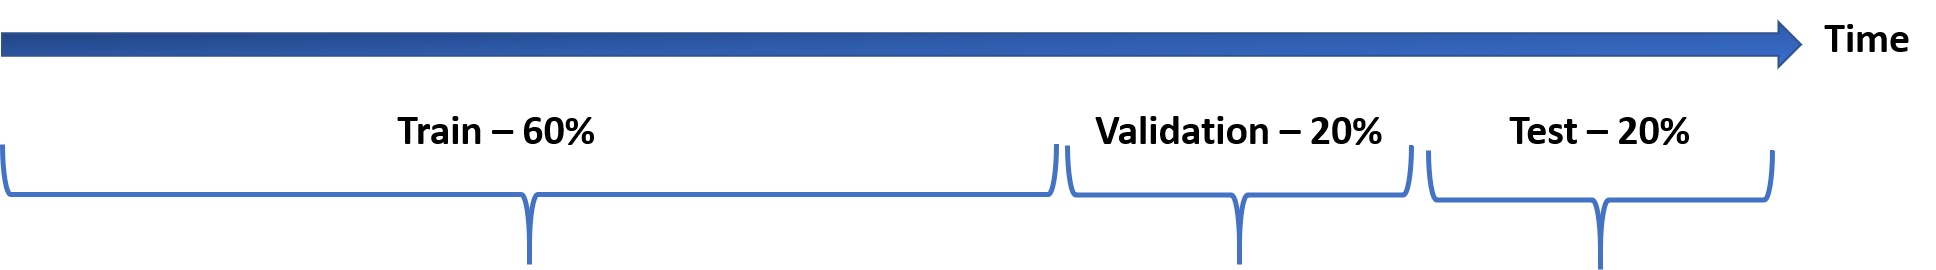
\includegraphics[width=1.0\textwidth]{Figures/seperation.png}\quad

\caption{Separation to train, validation, and test sets along the time of assigning USIs to a sprint}
\label{fig:train-test-separation}
\end{figure}

The train set is used for training the models, while the validation set used as the test set for features selection and tuning the hyper-parameters. After selecting the best features and parameters for the prediction models, we used the train and validation sets to train the models with the selected parameters and evaluate the results on the test set.
The test set is untouched in the features selection and tuning hyper-parameters stages, and use only for the evaluation of the results.



\subsection{Feature Extraction}
One of the main challenges of this work is to identify features (properties/characterizations) that relate to changes in the text, and would support the prediction of changes and alert on \emph{unstable} USIs at the time they are assigned to a sprint. 

In this work, we divided the sought features into four groups: simple text based features, advanced text based features, process-based features, and personalized features.

The first two groups refer to the text itself. For that purpose, we used the version of the text at the time it is assigned to a sprint. In case the text is missing or unclear, we expect it would probably change. In addition, some words may provide indication about the text quality. For example, text that contains question marks indicates uncertain and a discretionary request. Text without verbs at all may imply that it misses instructions to the developers. 

The different ML algorithms cannot understand the text in its original format, as the different letters or words alone without the context do not provide these with helpful information. Thus, there is a need to pre-process the text and then transform the text into numeric features that encapsulate its semantics. 

In addition, the raw text originating from the Jira is noisy and is different from one project to another. For example, one project is written in an HTML format, and hence, there is need to clean the redundant tags and remain with the text only. In other projects, there are headlines and formats that need to be removed. For this purpose the pre-processing is intended for text cleaning and for removing of irrelevant information from the text, such as URLs and code snippets. 

After pre-processing the text, we were able to derive its related features, as follows.


\paragraph{\textbf{Simple Text Based Features.}}
%The features in this group are directly derived from the text. These include the length of the text (long text might imply limited cohesion or missing information if it is too short), use of template, missing verbs, URL containment (this might indicate that the USI is not self contained) and the presence of a specific words, such as 'TBD'' in the text that may reflect on the USI stability. 
The features in this group are directly derived from the text, after a deep examination of the USIs and their various characteristics. %These include the length of the text (long text might imply limited cohesion or missing information if it is too short), use of template, missing verbs, URL containment (this might indicate that the USI is not self contained) and the presence of a specific words, such as “TBD” in the text that may reflect on the USI's stability.
\begin{itemize}
    \item Length of the text - short text can testify on missing details, and very long text can suffer from over details and limited cohesion and may cause confusion. It is calculated by counting the number of characters in the USI. For example, “UI: User should be able to get all the job executions on a given job at deployed jobs page. On clicking a specific job on the deployed jobs list, we need to redirect the user to show the list of all the job executions on that job. User should be able to navigate back to the deployed jobs list.” The length of this USI is 292.
    
    \item URL containment - URL can add additional information that is missing in the text. It is calculated by moving over the text and checking if it contains a URL address. If yes- the value is 1, else-0. For the USI example above, the value is 0, since it does not contain a URL.
    
    \item Special word containment - indicates of whether the text contains the words “TODO/TBD/Please” (yes or no). These words imply something missing or unclear in the text, with a high probability of editing and changing. It is calculated similar to the previous feature, except that we check the presence of the words “TODO”, “TBD” and “Please”. For the USI example above, the value is 0, since it does not contains these words.
\end{itemize}
%\newline
\paragraph{\textbf{Advanced Text Based Features.}}
The features in this group refer to various indicators resulted from applying various Natural Language Processing (NLP) techniques to extract relevant information. 

    \begin{itemize}
        \item Topic model - %we split the USI into topics, and add the feature of the topic to each USI. This feature may be able to identify important topics that might affect the USI stability.
        %[Arnon-this should be rephrased] -Yarden - I don't understand what is not clear in this paragraph, It's written as in the thesis.
        given the number of topics, it split the USIs into that number of topics, by the text similarity. In fact, every topic is a probability of all the corpus words, but to each topic that probability is different, and the highest probability words characterise the topic. For example, text that relates to medicine include the words Doctor, illness, and disease in the top probability words. We divided the USIs into groups to hopefully find the topics of the USIs. The topics of the USI can relate and affect the USI stability, USIs that relate to an important part in the software development may get more attention, and hence we will expect them to be in high quality and without any changes. We found to each project the best number of topics by the results on the validation set, and use it to the topic model. To each project, we train a topic model, and divide the USIs to the different topics, and added the topic as a feature. It is important to notice also in this algorithm, we learn the relations and the distribution of the topics by the train set and infer on the test set. We do not use the test set for creating the topic model.
         \item Document vector - translates the documents (USIs) text into a vector of numbers. The vector is used to represent the content and is calculated by learning the document embeddings via the distributed memory model  \cite{le2014distributed}. This model inspired by word embedding, where the document token can be thought as another word. The model acts as a memory that remembers what is missing from the current context or the topic of the document. The document vectors is trained using stochastic gradient descent and the gradient is obtained via back-propagation. We train our distributed memory model and learn the relations with the USIs' train set, and infer on the USIs' test set. For each project, we created a different model based on its own dictionary, and added this vector as a feature to the model.
           \end{itemize}
%\newline 
\paragraph{\textbf{Process-Based Metrics.}}
%All the information that the Jira tool provides us on the work process history and relations of the USI besides the text.
    
This feature group refers to text edits and setting, relations (such as issue links), and changes in the USI's fields before it is assigned to a sprint. The Jira tool document all the changes related to the USI from its creation. This includes all the comments as well as changes in its fields. We tracked the number of changes in the text and the comments that were added. Many changes or comments may indicate a problem with the USI. 
%Also, we tracked the priority, the story point and more. 

\begin{itemize}
    \item Number of changes in the text before entering a sprint - introducing many changes to a USI before it us assigned to a sprint can point to a problem with the text or unclear request, and can cause to more changes during the sprint. It is calculated similar to the stability calculation. The different is that we count only changes that happened before the USI is assigned to a sprint.
    \item Number of comments before entering a sprint - if a USI has many comments, it can indicate on an unclear request. We count only comments that were added before the USI is assigned to a sprint.
    \item USI priority - one influence of the priority can be, for example, if the USI is urgent, it may cause to fast and less strict writing, or the opposite, strict writing from the reason to be performed in the best way. Each USI contains the priority field, so we use the value of this field at the time the USI is assigned to a sprint.
\end{itemize}
    
%All these features relate to the stability of the USI, and contains important information that helps us to predict the changes.
%\newline
\paragraph{\textbf{Personalized Metrics.}}  
Another factor that may affect the USI stability is the author of the USI. Thus, the features in this group refer to the USI author’s history and experience. 

\begin{itemize}
    \item Author's number of USIs - The number of USIs that the author wrote before the current USI. The idea behind that feature is that we expect from a person with limited experience in writing USI, to write USI with limited quality. On the other hand, we expect that a skilled person, to write high quality USI, with a lower probability that the USI will be changed.
    \item Author's ratio of unstable USIs. The ratio of unstable USIs from all the USIs that the author wrote before the specific USI. We expect that the probability that a USI will be changed increase when the ratio of unstable USI to an author is high.
\end{itemize}

%Another factor that may affect on the USI stability is the author of the USI. Thus, the features in this group refer to the USI author's history and experience. We expect that experienced USI authors to write more \emph{stable} USI than those who had no experience and wrote only a few. We also expect that there is a correlation between the ratio of \emph{unstable} to \emph{stable} USIs of an author and the stability of the next USI written by the same author.

%This feature group consists of the following features: the number of USIs that the author wrote before the current US, and the ratio of \emph{unstable} USIs from all the USIs that the author wrote before the specific USI.

%[Arnon not sure it should be here] - I think this is the best place for it, we talk here on the features extraction, we detail about all the features groups and say how we chose these features to each project.
Having set the various feature groups, we turn into the selection of the best combination of these for each project separately, based on the train and validation set. 
We used the train and validation set, and for each project we extract the combination of the features groups that performed the best results on the validation set, and predict on the test set by these groups only. 
% For example, in \ref{features_groups_influence_subsection} we can see

%For example, table \ref{Table:feature groups validation} indicates that the best groups accepted for the commercial project is the groups of advanced text based features, simple text based features, and personalized metrics.

\subsection{Prediction Models}

For devising the predication models, we compared three state-of-the-art supervised learning algorithms that are commonly used for classification problems, similar to ours.

\begin{itemize}
    \item \textbf{Random Forest (RF)} is an ensemble of independent decision trees \cite{breiman2001random}. %It has high predictive accuracy and it can handle large data-set and multiple features. 
    \item \textbf{Neural Network (NN)} is a nonlinear model that consists of an input layer, hidden layers, and output layer \cite{bishop1995neural}. %It has the ability to learn nonlinear and complex patterns in the data, and can handle large data-sets \cite{bishop1995neural}. 
    In this study we used a multi-layer feed forward NN, where the number of layers and internal neurons in each layer was chosen by the hyper parameters optimization.
    \item \textbf{eXtreme Gradient Boosting (XGboost)} is an implementation of gradient boosted decision trees \cite{chen2016xgboost}. It was developed for improving model performance and computational speed. %It is fast learning and improves model accuracy. 
\end{itemize}

% For each algorithm we tuned the hyper-parameters by the results on the validation set.

Each algorithm has its characteristics and advantages, which can fit for our problem. The RF has high predictive accuracy and it can handle large data-set and multiple features, as we have in our work; The NN has the ability to learn nonlinear and complex patterns in the data, and can handle large data-sets; and the XGboost is fast learning and improves model accuracy. Hence, we chose to use these three algorithms and compare their results, to obtain as accurate results as possible. % For each algorithm, we tuned the hyper-parameters by the results on the validation set.


Each algorithm has several hyper-parameters that affect its performance. To select the parameters that improve the results we performed parameters optimization. For that purpose we used the train and validation sets and select the combination of parameters with
the best results of the area under the precision-recall curve on the validation set. We chose for each project and each label the best parameters separately.
The parameters we chose for the RF algorithm are the number of trees, max features and max depth of each tree to avoid over-fitting. The parameters we chose for the NN algorithm are hidden layer sizes (we tried different combinations of the number of layers and number of neurons in each hidden layer), activation functions, solver and the
learning rate. The parameters we chose for the XGboost algorithm are the number of trees, max depth of each tree, and the scale of %[Arnon??- Yarden I add explanation] 
positive weight, which is the ratio of number of negative class to the positive class, to deal with the imbalanced data.


%[Arnon - later in the results the values of the hyperparameters should be mentioned] -Yarden - there are a lot of values and I don't think adding them is relevant in the article, also in the thesis we didn't add them, This is minor information that usually don't added to articles.

\section{Results}
\label{sec-results}

Following the data collection and preparation, in this section, we present the results. We start with the general statistics, Next, we provide explanation for the evaluation measures. Then, we introduce the results of the prediction models in comparison to two baselines. Finally, we analyze the results and discuss the effects of the various features.
%the challenges arise from it. 
% Next, we explain the evaluation measures, followed by the analysis of the important features. Finally, compare results of the predicting models to two baselines.


\subsection{General Statistics}

First, we check the ratio between \emph{stable} and \emph{unstable} USIs in each one of the projects. Table \ref{Table:lable ratio} shows the ratio of the two types of unstable USI- changes in more than five words and changes in more
than twenty words, in all projects. %The rows represents the different projects, the second column represents the number of USIs in each project, the third column represents the number of \emph{unstable} USIs by the label of change in more than five words (and the brackets represent the percentage of these), and the last column represents the same, for the second label - change in more than twenty words.
It indicates that the data is imbalanced, for example, in the "XD" project there are 1741 USIs that are stable and only 80 USIs that are not. That is, most of the USIs are \emph{stable} and did not change during a sprint and the minority of the USIs are \emph{unstable} and were changed after they entered the sprint. This observation makes a perfect sense, because a change means instability, so we do not expect to see a lot of it. Referring to the open source projects, it is interesting to notice that the smaller projects have a higher ratio of \emph{unstable} USIs then the large projects. When comparing the commercial project to the open source projects, it seems that they have similar characteristics. 

%Having projects with different sizes, we are also able to check of whether the project size affect the resulting model.

%Another thing to notice from Table \ref{Table:lable ratio} is the different project sizes, from the small one - "REPO" with 900 USI to the large one - "DM"; In that way, we are able to examine our model on varied projects.

% label statistics ratio
\begin{table}[h]
    \centering
    \caption{List of the number of the two types of \emph{unstable} USI-
    changes in more than five words and changes in more than twenty words, in all the different projects (in brackets the percentage of these from all the USIs)}
    \begin{tabulary}{\textwidth}{lccc}
    \toprule
    %\cmidrule(rl){1-4}
    Project & \hfil \# of USI & \# \emph{unstable} USI-5 & \hfil \# \emph{unstable} USI-20\\
    %\midrule
    \cmidrule(rl){1-1}\cmidrule(rl){2-2}\cmidrule(rl){3-3}\cmidrule(rl){4-4}
      Commercial  & 1855 & 377 (20\%) & 235 (13\%) \\ 
      DEVELOPER   & 1229 & 394 (32\%) & 290 (24\%) \\
      REPO        & \phantom{0}900  & 195 (22\%) & 140 (16\%) \\
      XD          & 1741 & 173 (10\%) & 80 (5\%) \\
      DM          & 4962 & 626 (13\%) & 415 (8\%) \\
      \bottomrule
    \end{tabulary}
\label{Table:lable ratio}
\end{table}

Next, we were interested to see if the USI stability is affected by the format for writing USI. Table \ref{Table:ratio template_5} presents the descriptive statistics for changes in at least five words, where the results of changes in at least twenty words is presented in Table \ref{Table:ratio template_20} and are similar to the results in \ref{Table:ratio template_5}. Overall, it seems that using templates have similar affect on changes when ignoring the use of a template. For that reason, we analyze all USIs together. 


\begin{table}[]
	\centering
	\caption{Ratio between change in the text and text written by template - 5 words}	
    \begin{tabular}{lccc}
	\toprule
	
	Project	& 
	\multicolumn{1}{p{1.5cm}}{\centering \% with template \\ } &
	\multicolumn{1}{p{1.9cm}}{\centering \% with template \\ \& with change } &
	\multicolumn{1}{p{1.9cm}}{\centering \% without template \\ \& with change } \\
	
	%Project	&
	%\% with template & \% with template and with change &  \% without template and with change \\
	\midrule
	Commercial & \phantom{0}4.4\% & 30.0\%           & 20.0\%  \\
	DEVELOPER  & \phantom{0}3.0\% & 24.0\%           & 32.0\%  \\
	REPO	   & 15.2\%           & 34.0\%           & 24.0\%  \\
	XD	       & 17.0\%           & 20.0\%   & \phantom{0}8.0\% \\
	DM	       & \phantom{0}0.1\% & \phantom{0}0.0\% & 13.0\%  \\
	% \hline
	\bottomrule
    \end{tabular}
    \label{Table:ratio template_5}
\end{table}



\begin{table}[]
	\centering
	\caption{Ratio between change in the text and text written by template - 20 words}	
    \begin{tabular}{lccc}
	\toprule
	
	Project	& 
	\multicolumn{1}{p{1.5cm}}{\centering \% with template \\ } &
	\multicolumn{1}{p{1.9cm}}{\centering \% with template \\ \& with change } &
	\multicolumn{1}{p{1.9cm}}{\centering \% without template \\ \& with change } \\
	
	%Project	&
	%\% with template & \% with template and with change &  \% without template and with change \\
	\midrule
	Commercial & \phantom{0}4.4\%  & 15.6\%           & 19.6\%  \\
	DEVELOPER  & \phantom{0}3.0\%  & 13.5\%           & 23.9\%  \\
	REPO	   & 15.2\%           & 24.8\%           & 13.8\%  \\
	XD	       & 17.0\%           & 11.4\%   & \phantom{0}3.1\% \\
	DM	       & \phantom{0}0.1\% & \phantom{0}0.0\% & 8.3\%  \\
	% \hline
	\bottomrule
    \end{tabular}
    \label{Table:ratio template_20}
\end{table}


% \subsubsection{Relation between USI template and USI stability}
% We were further 



% ratio of stable and unstable in the test and train sets:
% We are also interested to verify that 
Next, we were interested to %verify that 
examine if the ratio between \emph{stable} and \emph{unstable} USIs in both the train and the test set is similar. Table \ref{Table:train test ratio} presents this ratio for both of the thresholds we defined. It indicates that the ratio of \emph{unstable} USIs in the commercial project is lower in about 10\% in the test set compared to the train set, and this hold for "DEVELOPER" project as well. On the other hand, in the "XD" project, the situation is opposite. %, as we expected. 

The different ratio between the train set and the test set affects the prediction task and makes it more challenging. 
The classification algorithms used for the task at hand learn about the future from past experience, and since we have different patterns, i.e., different ratio in the train and test set in several projects, it may interfere with the learning. We wish to overcome this using the features we defined. 



\begin{table}[]
    \centering
    \caption{List of the ratio of the two types of \emph{unstable} USI- 
    changes in more than five words and changes in more than twenty words, in the train vs test set in all the different projects}
    \begin{tabular}{l|c|c|c}
	 \toprule
     \multicolumn{4}{c}{train} \\
    \toprule
	Project & \hfil \# of USI & \# \emph{unstable} USI-5 & \hfil \# \emph{unstable} USI-20\\
	\hline
	Commercial  & 1483           & 335 (23\%)       & 217 (15\%) \\
      DEVELOPER & \phantom{0}983 &  334 (34\%)      & 247 (25\%) \\
      REPO      & \phantom{0}720 &  180 (25\%)      & 116 (16\%) \\
      XD        & 1393           & 122 \phantom{0}(9\%) & \phantom{0}49 \phantom{0}(4\%) \\
      DM        & 3970         & 509 (13\%) & 332 \phantom{0}(8\%) \\
	\toprule
     \multicolumn{4}{c}{test} \\
    \toprule
	Project & \hfil \# of USI & \# \emph{unstable} USI-5 & \hfil \# \emph{unstable} USI-20\\
	\hline
	  Commercial & 370 & \phantom{0}40 (11\%) & 17 \phantom{0}(5\%) \\ 
      DEVELOPER  & 246 & \phantom{0}60 (24\%) &  43 (17\%) \\
      REPO       & 180 & \phantom{0}48 (27\%) &  24 (13\%) \\ 
      XD         & 348 & \phantom{0}51 (15\%) &  31 \phantom{0}(9\%) \\
      DM         & 992 & 117 (12\%)           &  83 \phantom{0}(8\%) \\
      \toprule
    \end{tabular}
\label{Table:train test ratio}
\end{table}

%\begin{table*}[h]
 %   \centering
  %  \caption[train ratio]{List of the ratio of the two types of \emph{unstable} USI - changes in more than five words and changes in more than twenty words, in the train vs test set in all the different projects}
   % \begin{tabular}{c|c|c|c|c|c|c}
    %\toprule
	%Project & \hfil \# USI in train & \# USI in test & \# %\emph{unstable} USI-5 in train & \hfil \# \emph{unstable} USI-5 in test & 
	% \# \emph{unstable} USI-20 in train & \hfil \# \emph{unstable} USI-20 in test \\
%	\hline
	%Commercial & 1483 & 370 & 335 (23\%)& 40 (11\%) &  217 (15\%) &  17 (5\%)\\   
   %  DEVELOPER & 983 & 246 & 334 (34\%)&60 (24\%) & 247 (25\%)    & 43 (17\%)\\ 
    % REPO   & 720 & 180 & 180 (25\%)&48 (27\%) & 116 (16\%) & 24 (13\%) \\       
    % XD       & 1393 & 348 & 122 (9\%)&51 (15\%)& 49 (4\%)  & 31 (9\%)\\  
    % DM      & 3970 & 992  & 509 (13\%)& 117 (12\%)& 332 (8\%)&  83 (8\%)\\ 
     % \toprule
    %\end{tabular}
%\label{Table:train test ratio2}
%\end{table}

% We are also interested in examining the number of changes along the time after entering a sprint. 
%For that purpose, we first study when most of the changes happen, and second we study the ratio between \emph{stable} and \emph{unstable} USI throughout the development time.

We were also interested in examining the number of changes along the time after entering a sprint. This information can help us understand the work process, when most changes occur and the behavior of the changes during the sprint. Figure \ref{fig:changes after sprint} presents the number of changes in USIs in the first two weeks after the USIs enter the sprint, for all the different projects. It is evident that most of the changes happen in the first day of the sprint for all the projects, and there are fewer changes as the sprint progress. These results are not surprising, as on the first day, the developers start working on the USIs that were added to the current sprint. Thus, if something is not clear, the higher probability it comes up during this time. Our goal is to lower the amount of changes during this time frame by predicting such unstable USIs, so developers are able to move into implementation as soon as possible. 

\begin{figure}[ht]
\centering
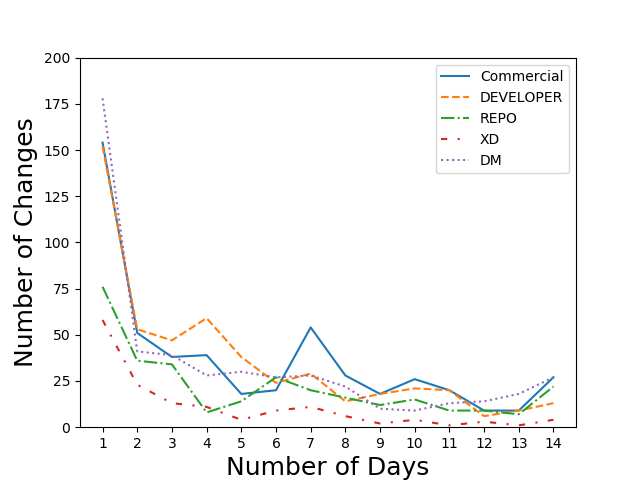
\includegraphics[width=.45\textwidth]{Figures/number_changes_after_sprint_two_weeks_only_new.png}\quad

\caption[Number changes two weeks]{\centering Number of changes after the sprint started in the first two weeks}
\label{fig:changes after sprint}
\end{figure}



\subsection{Evaluation Metrics}

In evaluating prediction problem (as in our case), it is common to refer to four possible metrics: True Positives (TP), False Negatives (FN), False Positives (FP) and True Negatives (TN). In our context, TP refers to USIs that changed after they entered the sprint (i.e., are unstable), and the model predicted these correctly. FP refers to USIs that did not change after they entered the sprint (i.e., are stable), and the model predicted these as unstable. FN refers to USIs that changed after they entered the sprint (i.e., are unstable), and the model predicted these as stable. TN refers to USIs that had not been changed after they entered the sprint (i.e., are stable), and the model predicted these as unstable.

We use the confusion matrix that consists of the four metrics and evaluate the model performance by three different measures: accuracy, the area under the Receiving Operating Characteristics (ROC) curve and area under the precision-recall curve. 
%[Arnon -maybe present these matrix in the appendix, they can be used for further analysis] Yarden - I don't think it's a good idea since we talked about it that the accuracy is not a good measure because it relate to a specific threshold (and so is the matrix, the accuracy calculated by the confusion matrix), and that the reason we chose to use ROC and pre-recall curve, these measures also relates to the FP,FN,TP,TN. 
%The accuracy measure relates to the final classification, according to a specific threshold, and provides an initial evaluation. 
The accuracy is the ratio between the number of correct predication and the total number of USIs (correct predication and wrong predication):
\begin{equation}
        Accuracy = \frac{TP + TN}{TP+TN+FP+FN}
\end{equation}

However, our data is imbalanced, meaning that most of USIs did not change, and only a small percentage of them had changed. In that case, even if we predict that all the stories will not change, the accuracy of the algorithm will be high, so we need metrics that take the imbalance into account. 

For that purpose, we used the other two measures that relate to the different thresholds and indicate of how much the model is capable of distinguishing between the cases of stability.

The first measure is the area under the receiver operating characteristic (ROC) curve, which is the trade-off between the true positive rate (TPR) and false positive rate (FPR) at various thresholds settings. Larger area under the ROC curve indicates better predication. When the area under the curve is 1, it means a perfect model. When the area under the curve is 0.5, it means the model has no ability to distinguish between the stability cases.

TPR is defined as:
    \begin{equation}
        TPR = \frac{TP}{TP+FN}
    \end{equation}

FPR is defined as:
    \begin{equation}
        FPR = \frac{FP}{FP+TN}
    \end{equation}
    
The second measure is the area under the precision-recall curves, which is the trade-off between the precision and recall using different probability thresholds. Here again, larger area under the precision-recall curve indicates better predication. The area under the precision-recall curves take into account the imbalanced of the two stability cases and hence is very useful for the evaluation of imbalanced data, and it is the most important measure in our study. The recall is the TPR as defined in equation 2. A poor classifier will be a horizontal line on the plot with a precision that is proportional to the number of positive examples in the data, and when the area under the curve is 1, it means a perfect model.


Precision is defined as: 
    \begin{equation}
        Precision = \frac{TP}{TP+FP}
    \end{equation}


\subsection{Predication Results}

To examine the prediction results of achieved by the classification algorithms (after all optimization were made) we compare the results with two baselines: random prediction and a prediction in which all USIs are stable (as these are the majority). 
Table \ref{Table:prediction results 5} presents the results of USI stability prediction (when referring to changes in at least five words after the USI enters the sprint), by the two baselines: random predication (Rnd) and predict all to be stable (Maj), and the three classification algorithms: Random Forest (RF), Neural Network (NN) and XGboost (XG), according to three measures: area under precision-recall curve (AUC PRC), area under the ROC curve (AUC ROC) and the accuracy (Acc). The best results for each project by each one of the measures is marked in bold.

The predication models we developed improve the baseline results in more than 10\% in all five projects. The Random Forest model achieved the best results in the open-source projects, and the Neural Network model achieved the best results for the commercial project. This can be explain by the fact that the RF classifier can handle high dimensional data and achieve better results with a large number of features, as in the case of the open-source projects.

With respect to Accuracy (Acc), the developed predication models outperform the Random classifier (Rnd). However, the Majority baseline mostly achieve better results. This is not surprising, as we mentioned before, the data is imbalance and most of the USIs did not change. Yet, predicting all USIs as stable would not support the development process. Our main interest is to identify the unstable ones and in that sense the developed model is better. Furthermore, we notice that the Accuracy(Acc) of the developed predication models is almost the same as the Majority classifier and even higher in the commercial project, where the average Acc of all project by the RF classifier is 81\%, in contract to 82\% for the Majority baseline. Comparing the results to the Rnd baseline, we achieve an improvement of more than 15\% 
for each one of the projects. This indicates that the accuracy of the developed predication models is satisfactory. In particular, the developed classifier is better in finding the \emph{unstable} USIs.


Table \ref{Table:prediction results 20} is the similar to Table \ref{Table:prediction results 5}, except that it presents the stability prediction results based on changes in at least twenty words after the USI enters the sprint. The results are similar to the results in Table \ref{Table:prediction results 5}. With respect to the AUC PRC and AUC ROC measures, the developed prediction models improved the baseline results in more than 9\% for each one of the projects.
With respect to accuracy, the best results are achieved by the Majority classifier, whereas the RF and NN classifiers results are close or equal to the Majority baseline results. 

Among the three predication models, following the AUC PRC and AUC ROC measures, the RF achieved the best results for the most projects. In contrast to the results in Table \ref{Table:prediction results 5}, the best results for the commercial project were achieved by the RF classifier and for the "REPO" open-source project by the NN classifier.

As we said before, the RF classifier performs well with high dimensional data \cite{caruana2008empirical} as reflected in other classification problems in various domains \cite{chen2012random}. It achieved the best results for almost all the projects and the different measures. It might be that in the predictions in which the NN outperform the RF classifier results, the network succeeds to learn some complex relations that the RF had missed.

Examine the RF classifier results, the average AUC PRC of all project is 0.25, the average AUC ROC of all project is 0.72 and the Acc of all the project is above 80\%, with an average of 88\%. It is evident that the average AUC PRC is lower and the average Acc is higher, compared to Table \ref{Table:prediction results 5}. This is a result of the increased imbalance in the data, i.e., the percentage of the unstable USIs is decreased.

When the imbalance in the data increases, it is more difficult to identify the small group, the \emph{unstable} USIs in our case, and hence we were expecting to have lower AUC PRC. In addition, since we have less USIs that have changed in at least twenty words compare to USIs that have changed in at least five words, the accuracy increase, because the change in at least twenty words is less common and the number of USIs that change is smaller. Table \ref{Table:prediction results 20} approves the results as we expected. It also demonstrates that the developed predication models overcome the baseline results.

%\begin{table*}[h]
%	\centering
%	\caption{Stability Prediction - change in 5 words: 
%	by two baselines- random classification (Rnd) and predict all to be stable, the majority (Maj), and three learning algorithms- Random Forest (RF), Neural Network (NN) and XGboost (XG), according to three measures- area under precision-recall curve (AUC PRC), area under the ROC curve (AUC ROC) and the accuracy (Acc)}	
    
            
%    \begin{tabular}{|l|c|c|c|c|c|c|c|c|c|c|c|c|c|c|c|}
%	 \hline
 %   {} &  \multicolumn{5}{|c|}{AUC PRC} & \multicolumn{5}{|c|}{AUC ROC} & \multicolumn{5}{|c|}{Acc} \\
  %  \hline
%	Project	&      Rnd &  Maj &  RF  &  NN  &  XG  & Rnd  & Maj &  RF  &  NN  &  XG  & Rnd & Maj &  RF  &  NN  & XG  \\
%	\hline
%	Commercial	&  0.11 & 0.11 & 0.29 & \textbf{0.30} & 0.26 & 0.50 & 0.50 & 0.73 & \textbf{0.76} & 0.73 & 0.49 & 0.89 & \textbf{0.90} & 0.88 & 0.74 \\
%	DEVELOPER	&  0.27 & 0.24 & \textbf{0.40} & 0.35 & 0.35 & 0.50 & 0.50 & \textbf{0.64} & 0.57 & 0.60 & 0.52 & \textbf{0.76} & 0.75 & 0.75 & 0.66 \\
%	REPO	    &  0.31 & 0.27 & \textbf{0.41} & 0.38 & 0.31 & 0.54 & 0.50 & 0.69 & \textbf{0.70} & 0.59 & 0.53 & \textbf{0.73} & 0.69 & 0.69 & 0.59 \\
%	XD	        &  0.20 & 0.15 & \textbf{0.40} & 0.34 & 0.30 & 0.57 & 0.50 & \textbf{0.76} & 0.74 & 0.71 & 0.57 & \textbf{0.85} & 0.84 & \textbf{0.85} & 0.61 \\
%	DM	        &  0.12 & 0.12 & \textbf{0.26} & 0.24 & 0.22 & 0.52 & 0.50 & \textbf{0.72} & 0.70 & 0.69 & 0.52 & \textbf{0.88} & \textbf{0.88} & \textbf{0.88} & 0.86 \\
%	\hline
 %   \end{tabular}
  %  \label{Table:prediction results 5 1}
%\end{table*}



%\begin{table*}[h]
%	\centering
%	\caption{Stability Prediction - change in 20 words:
%	by two baselines- random classification (Rnd) and predict all to be stable, the majority (Maj), and three learning algorithms- Random Forest (RF), Neural Network (NN) and XGboost (XG), according to three measures- area under precision-recall curve (AUC PRC), area under the ROC curve (AUC ROC) and the accuracy (Acc)}		
    
 %   \begin{tabular}{|l|c|c|c|c|c|c|c|c|c|c|c|c|c|c|c|}
	 
%	 \hline
 %   {} &  \multicolumn{5}{|c|}{AUC PRC} & \multicolumn{5}{|c|}{AUC ROC} & \multicolumn{5}{|c|}{Acc} \\
  %  \hline
%	Project	&      Rnd & Maj &  RF   &  NN  &  XG  & Rnd  & Maj &  RF  &  NN  &  XG  &  Rnd & Maj &  RF  &  NN  & XG  \\
%	\hline
	
%	Commercial	&  0.05 & 0.05 & \textbf{0.31} & 0.24 & 0.27 & 0.50 & 0.50 & \textbf{0.87} & 0.86 & 0.84 & 0.52 & \textbf{0.95} & \textbf{0.95} & 0.94 & 0.87 \\
%	DEVELOPER	&  0.15 & 0.17 & \textbf{0.34} & 0.31 & 0.29 & 0.46 & 0.50 & 0.67 & 0.58 & \textbf{0.68} & 0.46 & \textbf{0.83} & 0.80 & \textbf{0.83} & 0.75 \\
%	REPO	    &  0.14 & 0.13 & 0.16 & \textbf{0.22} & 0.14 & 0.45 & 0.50 & 0.58 & \textbf{0.71} & 0.53 & 0.55 & \textbf{0.87} & 0.84 & 0.83 & 0.68 \\
%	XD	        &  0.09 & 0.09 & \textbf{0.23} & 0.14 & 0.19 & 0.45 & 0.50 & \textbf{0.77} & 0.61 & 0.68 & 0.49 & \textbf{0.91} & 0.90 & \textbf{0.91} & 0.89 \\
%	DM	        &  0.10 & 0.08 & \textbf{0.23} & 0.22 & 0.16 & 0.51 & 0.50 & \textbf{0.71} & 0.70 & 0.68 & 0.49 & \textbf{0.92} & \textbf{0.92} & 0.91 & 0.90 \\
	
%	\hline
 %   \end{tabular}
  %  \label{Table:prediction results 20 1}
%\end{table*}


\begin{table*}[h]
	\centering
	\caption{Stability Prediction - change in 5 words: 
	by two baselines- random classification (Rnd) and predict all to be stable, the majority (Maj), and three learning algorithms- Random Forest (RF), Neural Network (NN) and XGboost (XG), according to three measures- area under precision-recall curve (AUC PRC), area under the ROC curve (AUC ROC) and the accuracy (Acc)}	
    %\hline
            
    \begin{tabular}{|l|c|c|c|c|c|c|c|c|c|c|}
	 \hline
    {} &  \multicolumn{5}{|c|}{AUC PRC} & \multicolumn{5}{|c|}{AUC ROC}  \\
    \hline
	Project	&      Rnd &  Maj &  RF  &  NN  &  XG  & Rnd  & Maj &  RF  &  NN  &  XG  \\
	\hline
	Comme.	&  0.11 & 0.11 & 0.29 & \textbf{0.30} & 0.26 & 0.50 & 0.50 & 0.73 & \textbf{0.76} & 0.73  \\
	DEVE.	&  0.27 & 0.24 & \textbf{0.40} & 0.35 & 0.35 & 0.50 & 0.50 & \textbf{0.64} & 0.57 & 0.60  \\
	REPO	    &  0.31 & 0.27 & \textbf{0.41} & 0.38 & 0.31 & 0.54 & 0.50 & 0.69 & \textbf{0.70} & 0.59  \\
	XD	        &  0.20 & 0.15 & \textbf{0.40} & 0.34 & 0.30 & 0.57 & 0.50 & \textbf{0.76} & 0.74 & 0.71 \\
	DM	        &  0.12 & 0.12 & \textbf{0.26} & 0.24 & 0.22 & 0.52 & 0.50 & \textbf{0.72} & 0.70 & 0.69  \\
	
	\hline \hline
	{} &  \multicolumn{5}{|c|}{Acc}\\
	
	\cmidrule{1-6}
	%\hline{1-6}
	Project	    &   Rnd & Maj &  RF  &  NN  & XG \\
	\cmidrule{1-6}
	%\hline
	Comme.	& 0.49 & 0.89 & \textbf{0.90} & 0.88 & 0.74 \\
	DEVE.	& 0.52 & \textbf{0.76} & 0.75 & 0.75 & 0.66 \\
	REPO	    & 0.53 & \textbf{0.73} & 0.69 & 0.69 & 0.59 \\
	XD	        & 0.57 & \textbf{0.85} & 0.84 & \textbf{0.85} & 0.61 \\
	DM	        & 0.52 & \textbf{0.88} & \textbf{0.88} & \textbf{0.88} & 0.86 \\
	\cmidrule{1-6}
	%\hline
    \end{tabular}
    \label{Table:prediction results 5}
\end{table*}


\begin{table*}[h]
	\centering
	\caption{Stability Prediction - change in 20 words:
	by two baselines- random classification (Rnd) and predict all to be stable, the majority (Maj), and three learning algorithms- Random Forest (RF), Neural Network (NN) and XGboost (XG), according to three measures- area under precision-recall curve (AUC PRC), area under the ROC curve (AUC ROC) and the accuracy (Acc)}		
    %\hline
    \begin{tabular}{|l|c|c|c|c|c|c|c|c|c|c|}
	 % \toprule
	 \hline
    {} &  \multicolumn{5}{|c|}{AUC PRC} & \multicolumn{5}{|c|}{AUC ROC}   \\
    \hline
	Project	&      Rnd & Maj &  RF   &  NN  &  XG  & Rnd  & Maj &  RF  &  NN  &  XG    \\
	\hline
	% \textbf
	Comme.	&  0.05 & 0.05 & \textbf{0.31} & 0.24 & 0.27 & 0.50 & 0.50 & \textbf{0.87} & 0.86 & 0.84  \\
	DEVE.	&  0.15 & 0.17 & \textbf{0.34} & 0.31 & 0.29 & 0.46 & 0.50 & 0.67 & 0.58 & \textbf{0.68}  \\
	REPO	    &  0.14 & 0.13 & 0.16 & \textbf{0.22} & 0.14 & 0.45 & 0.50 & 0.58 & \textbf{0.71} & 0.53  \\
	XD	        &  0.09 & 0.09 & \textbf{0.23} & 0.14 & 0.19 & 0.45 & 0.50 & \textbf{0.77} & 0.61 & 0.68  \\
	DM	        &  0.10 & 0.08 & \textbf{0.23} & 0.22 & 0.16 & 0.51 & 0.50 & \textbf{0.71} & 0.70 & 0.68  \\
	
	\hline \hline
	{} &  \multicolumn{5}{|c|}{Acc}\\
	\cmidrule{1-6}
	%\hline
	Project	    &   Rnd & Maj &  RF  &  NN  & XG \\
	\cmidrule{1-6}
	%\hline
	Comme.	&   0.52 & \textbf{0.95} & \textbf{0.95} & 0.94 & 0.87 \\
	DEVE.	&   0.46 & \textbf{0.83} & 0.80 & \textbf{0.83} & 0.75 \\
	REPO	    &   0.55 & \textbf{0.87} & 0.84 & 0.83 & 0.68 \\
	XD	        &   0.49 & \textbf{0.91} & 0.90 & \textbf{0.91} & 0.89 \\
	DM	        &   0.49 & \textbf{0.92} & \textbf{0.92} & 0.91 & 0.90 \\
	\cmidrule{1-6}
	%\hline
    \end{tabular}
    \label{Table:prediction results 20}
\end{table*}
%[Arnon] in case we claim that our main interest is to identify unstable USIs - perhaps we can present these numbers.... Yarden, we present it in the tables.


\subsection{Features Groups Effect}
\label{features_groups_influence_subsection}
One of the goals of this work is to identify the features that affect the USI stability. For that purpose, we chose for each project the best fitted feature groups by the results on % applying the models to 
the validation set. 
% The chosen feature groups for each project are:

The chosen feature groups for each project present in Table \ref{Table:feature groups validation}, where the rows represents the projects, the columns represents the four feature groups and the "\checkmark" inside the table represents the chosen groups. For example, the best result for the "DM" project  were achieved using all of the four feature groups together.

The results indicate that each project has a different combination of groups, the Personalized Metrics affect the results in all projects and that Process Based Metrics affects the results in all open-source projects. 
In addition, the NLP-based features group affects the results of the commercial project, and besides of the "DM" project, it does not affect the results of the open-source projects. 

Furthermore, the "DM" project requires all feature groups to reach the best results. This can relate to the fact that the prediction results of this project are the lowest, which indicates that the models could distinguish between \emph{stable} and \emph{unstable} USIs only to a limited extent. Thus, every feature that we added improved the results, and every feature that we removed negatively affected the results. Examining the USIs in this project, we notice that they are written in a polite and %respectful
unofficial language, like using the words "please", "nice" and "great" in the text. For example: \emph{"Please install v14.0 in the shared stacks on lsst-dev. The stack release v14.0 just came out. It would be useful if v14.0 is available in the shared stack on lsst-dev."}
This might restrict the model ability to classify the USI stability to a satisfactory level.

\begin{table}[ht]
	\centering
	\caption{Feature Groups with the Best Results on the Validation Set.
	Where A-Advanced Text Based Features, B - Simple Text Based Features, C - Process Based Metrics, D - Personalized Metrics}

\begin{tabular}{l|c|c|c|c}
%\hline
	Project  &   A & B & C & D  \\ 
	\specialrule{.2em}{.1em}{.1em}
	Commercial & \checkmark  &\checkmark &            &\checkmark \\ \hline
	DEVELOPER  & 		     &\checkmark &\checkmark &\checkmark \\  \hline
	REPO       &             &           & \checkmark &\checkmark  \\ \hline
	XD         & 		     &            &\checkmark & \checkmark\\ \hline
	DM         &  \checkmark &\checkmark  &\checkmark & \checkmark \\ \hline
	%\hline
	\end{tabular}
	\label{Table:feature groups validation}
\end{table} 

After the prediction task, we also wanted to check the effect of the chosen features groups on the test set. For that purpose, we evaluated the results for each project with each of the chosen groups separately. For each of the projects, the results achieved by selecting all the groups together outperformed the results achieved when selecting each of the feature group separately. 

When comparing each one of the group separately, the feature groups that achieved the highest performance between the groups for each project are the following:

%[Arnon - can we have numbers here?, maybe for each project order the FG by their importance.] - I didn't save this information.

\begin{itemize}
    \item Commercial - simple text based features.
    \item DEVELOPER - simple text based features.
    \item REPO - process based metrics.
    \item XD - process based metrics.
    \item DM - personalized metrics.
\end{itemize}

These findings support the results accepted from the validation set and indicates uniformity. As we mentioned before, within the commercial project the text features are important, whereas in the open-sources projects the process based metrics have more influence; But also for them, the text is important as we notice in the "DEVELOPER" project. Referring to the "DM" project, the most important feature group is the personalized metrics. This may be derived from the reason that the text in this project is written in a less formal way and therefore has lower impact on the changes.

%[Arnon - do we have an analysis of each feature impact?] Yarden - No

\section{Discussion}
\label{sec-discussion}
%[Arnon - in the discussion we should elaborate on the results and their implications. For example, what are the important features and how can we justify this. Can we infer something from the project metadata? Yarden - We didn't enter this information to the article, so we can't write it in the discussion, and I don't save the information about each feature, we only looked for the best features group. maybe we can combine the discussion conclusions sections.
%[Yuval] I suggest we will start the discussion with a general statement about our study, before we go into the details 
From the general statistics we learned about the imbalance data and the differences between the train and test set. In addition, we notice that most of the changes in the USIs are introduced in the first days of the sprint, when the developers start working on it, so then the problems occur. 
%Also, we learned that there is a difference between the open-source projects and the commercial one in the content of the ratio between \emph{unstable} and \emph{stable} USs during the time. In the commercial project there is a learning curve, wherein the open-source projects, there is no significant difference along the different months. An explanation to this can be the different development process; In commercial projects, the work is done in teams located together, and in open source projects, the work is done remotely and the teams usually changed more frequently. 

For the prediction task we presented a classifications models that outperform the baseline results and improve the ability to identify \emph{unstable} USIs.
In addition, the results indicate that using the RF classifier achieved the best performance.

From the analysis of the features effect, we found out that there is a difference between the feature groups that affect the open-sources and the commercial projects, where the process-based metrics affect the open-sources projects and the advanced text based metrics affect the commercial project.
These results may be due to the fact that the team in the commercial project work together with daily Scrum meeting, had limited need to update information in the Jira, whereas the open source teams that are working in remote places needed to update information in the Jira to communicate effectively. Therefore, the features relate to the process-based and that passed through the Jira, had higher impact on the USI stability in the open-source projects. In the commercial project they had limited impact, and the text and related features had higher impact.   


%In this work we explored a novel impact-driven approach for assessing user stories. Several metrics for assessing a user story were proposed and discussed, based on the impact of the user story on the development process. We focused on a specific metric called stability, where a stable user story is one that does not change during the sprint in which it is implemented. To support the development process and identify problems in user stories before they enter a sprint, we apply machine learning approach to develop a model for predicting the stability of user stories. By identifying these user stories earlier in the development process, they could be further improved and elaborated, decreasing the chance for wrong implementation and wasted efforts during the sprint. We evaluated the prediction model on several open source and commercial projects. The results indicate that the model improved the baselines results significantly. It improved the results by more than 6\% in terms of PRC and ROC, with an average improvement of 15\% for all the projects in term of PRC, and with an average improvement of 20.6\% for all the projects in term of the ROC. This suggests that the prediction model can be used as a foundation of an advanced user story authoring system that will better support the software development process. 



\section{Threats to Validity}
\label{sec-threattovalidity}

%\textbf{Threats to Construct Validity}-
One of the threats is the inadequate operation of the independent variable, as lack of impact of the independent variable. To overcome this threat, we consulted with experts and studied the factors that affect USI stability from the data and the development process.

%\textbf{Threats to Internal Validity}-
Another threat is the ability of the classifiers to learn how to classify the \emph{unstable} USI, the ones that had changed after enters the sprint, since our data is imbalance. The percentage of \emph{unstable} USI are between 5 to 32. This is the statistics in the real world, so to deal with this threat, we used an evaluation measure that fit imbalance data - the area under the precision-recall curve. 

Another threat to validity is the selection bias which may occur due to the selection of the projects. This might affect the generalization of the results. To mitigate that threat we chose open-source projects with different sizes and from different repositories. We did not look for specific characteristics of projects. % In addition, we evaluate also a commercial project. 
Yet, it is required to apply and check the developed classifiers in other projects as well.
%[Yuval] it seems that something is missing here 

%\textbf{Threats to External Validity}- 
% which the results of an empirical investigation can be generalized to and across individuals, settings, and times.

%One of the threats to external validity is which the results of the study can be generalized to other software development projects. To face with that threat, we evaluate the results also on a commercial project besides the open source projects, since they have different work process.
%In addition, we used several open-source projects which are in different sizes and duration.
 

%One of the threats is the possibility %ability
%to generalize the study results on other software development projects. To minimize the threat we evaluate the results not only on open sources projects, but also on a commercial project, which have different work process. In addition, we used several open-source projects which are in different sizes and duration.


\section{Conclusion and Future Work}
\label{sec-conclsion}

In this paper we explored a novel data-driven approach for assessing USs. Several metrics for assessing USs were proposed and discussed, based on the impact of the US on the development process. We focused on a specific metric called stability, where a stable US is one that does not change during the sprint in which it is implemented. 

To support the development process and identify problems in USs before they enter a sprint, we apply machine learning to train a model that predicts USs stability. By identifying these USs earlier in the development process, they could be further improved and elaborated, decreasing the chance for wrong implementation and wasted efforts during the sprint.

We evaluated our prediction model on several open source and commercial projects. The results indicate that our model improved the random baseline results by more than 9\% in terms of AUC PRC and AUC ROC, for all the projects. This suggests that our prediction model can be used as a foundation of an advanced US authoring system that will better support the software development process. 

% We found out that the impact of the different feature groups varies greatly between projects, where process-based metrics is mainly noticeable within the open-source projects, and the effect of the advanced text based metrics is noticeable within the commercial project.

% We found out that one of the most important features for predicting stability, which relates to personalized metrics (that refer to the US's author experience), affects on the USI stability in all projects. Other features that affect the USI stability prediction refer to process-based metrics. This is mainly noticeable within the open-source projects. However, the effect of the advanced text based metrics is noticeable within the commercial project.

% The impact of the different features varies greatly between projects, suggesting directions for future research. 
 
In the future, we plan to improve the predicting results by using more advanced NLP tools, explore other features, and test other suitable classifiers. In addition, we aim to further examine the different impact of the feature groups between the projects. We are also interested in applying the classifiers to other commercial and open-source projects. 

%In the future, we plan to improve the predicting results by using more advanced NLP tools, explore other features, and test other suitable classifiers. We are also interested in applying the classifiers to other commercial and open-source projects.

% \begin{acks}
% %This research was supported by the Ministry of Science \& Technology, Israel.
% \end{acks}



















%%%%%%%%%%%%%%%%%%%%%%%%%%%%%%%%%%%%%%%%%%%%%%%%%%%%%%
%%%%%%%%%%%%%%%%%%%%%%%%%%%%%%%%%%%%%%%%%%%%%%%%%%%%%%
%%%%%%%%%%%%%%%%% old section 4 %%%%%%%%%%%%%%%%%%%%%%%%%%%%%%%%
%%%%%%%%%%%%%%%%%%%%%%%%%%%%%%%%%%%%%%%%%%%%%%%%%%%%%%
%%%%%%%%%%%%%%%%%%%%%%%%%%%%%%%%%%%%%%%%%%%%%%%%%%%%%%

% \section{Impact-Driven Approach to Assess User Stories}

%A major challenge in evaluating USs is to find the proper metrics.
%According to previous studies, the most prevalent template of USs is the one presented in the previous section \cite{lucassen2016use}, and many studies that define quality criteria rely on this template. 

%However, in the data set we derived from several projects, we %also notice the same phenomena notice that the template is not widely used. Table \ref{Table:ratio template} indicates that most of the projects do not follow the rules, and very few USIs follow that template. In three of the projects, less than 5\% follow the template, and for the remaining two, less than 20\% follow the template. 
%Yet, as we mentioned before, even if the USI contains the template and stands with the quality criteria defined in previous studies, it may still be misunderstood by the developers, or the other way around, it will be perfectly understood though it does not follow some of the quality criteria. 

%Following this situation, we seek for alternatives impact driven metrics for evaluating USs. 
%We looked for best practices, one of which refer to the fact that a US is assigned to a sprint only after it is well written and ready to execute \cite{buglione2013improving}. 
 %The metrics we examined will be detailed next and defined as follow: 

%\begin{itemize}
 %   \item Missing text fields
  %  \item Multiple sprints
%    \item Change in the story point after the USI enter the sprint
%    \item Change in the text after the USI enter the sprint
%\end{itemize}
%Changes in a US may imply that it was not well defined due to misunderstanding of the requirements, includes ambiguities, or lacks of enough details. Other possible metric is the number of sprints in which the US was assigned to. Multiple sprints for a specific US may imply that it was not well defined or included too much functionality. We also note that in many USs many details are missing, which may indicate that the US was not well defined. The last possible metric refers to changes in the story point (SP) after the US issue is assigned to the sprint. Since we do not expect to see changes in the US issue after it is assigned to the sprint, we do not expect a change in the SP field either. 

%In this section we will examine several data-oriented metrics


%Table \ref{Table:metrics statistics222} presents the descriptive statistics of the metrics we define above for the projects we examined. In the table columns represent the projects, the rows represent the metrics, and the cell represents the percentage of USI that fits each metric.

%\begin{table}[H]
%	\centering
%	\caption{Metrics Statistics- The percentage of USI by each metrics in all projects}
	
 %   \begin{tabular}{lccccc}
 %   \toprule
	%Metric	&	    Commercial   &  DEVELOPER  &  REPO    &    XD    &  DM     \\
%	\midrule
%	Missing text fields  & 24.1\%  &  15.3\% &  22.2\%  &  19.4\%  &  11.4\%  \\
%	Multiple sprints  & 10.1 \% &  41.1\% &  28.8\%  & \phantom{0}4.4\%   &  33.6\%  \\
%%%    \end{tabular}
    
%    \label{Table:metrics statistics222}
    % the table presents the percentage of USI that follow the condition
%\end{table}

%In the following, we explain and discuss each of the metrics. 

%\subsection{Missing text fields}

%We noticed that in many USs many details are missing, which may indicate that the US was not well defined. Following an expert interview, we understood that the Jira's fields of "summary", "description" and "acceptance criteria", should not remain empty. Nevertheless, in open source projects, we found out that the field "acceptance criteria" is not required and thus we have ignored this field in these projects. However, when referring to the commercial project, this field is very important and we include it in our calculation.  
%
%The metric relates to a USI that contains one or more empty text field at the time it enters to the sprint. Such USIs are missing relevant information, and therefore it can be considered as an assessment metric for USIs. Table \ref{Table:metrics statistics222} indicates that each project contains between 11 to 24 percentage of USIs with an empty fields, and the commercial project has a higher percentage.   

% why not good: 
%However, we noticed that in many closed USIs, those fields remain empty. This may indicate that the other fields contain the required information for the developers, and the metric of empty fields does not perfectly fit for the assessment of the USIs.

%\subsection{Multiple sprints}


%This metric relates to the number of sprints in which the US was assigned to. A USI should be a short requirement that suppose to be completed during a single sprint. %Multiple sprints for a specific US may imply that it was not well defined or included too much functionality.
%Hence, if a USI last more than one sprint and it is assigned to another one, this could indicate that the requirement described was too long and maybe it should have split into a few small requirements. Another reason that a USI lasts more than one sprint can be that the text was not understood and thus caused to delays. Table \ref{Table:metrics statistics222} indicates that each project contains between 4 to 41 percent of USIs that last more than one sprint. In the "XD" project, the percentage is the lowest, and most of the USIs last only one sprint, whereas in the "DEVELOPER" project, almost half of the USIs last more than one sprint.  

%The problem with that metric is that the multiple sprints do not necessarily point out a problem of the USI. It might be that the requirements were hard to implement or there was a need to execute other urgent stories instead, so it was postponed to next sprint. For these reasons, we chose not to use this metric. 

%\subsection{Change in the story point after the USI enter the sprint}

% A story point (SP) is a unit measure that is used for evaluating the development efforts that are required to complete the US. 
%This metric refers to changes in the story point (SP) after the USI is assigned to the sprint. When writing a USI, it common to add also the story points (SP) that take to implement it.
%As was said before, since the US is assigned to a sprint only after it is well written and ready to execute, we do not expect to see changes after it assigned to a sprint; so we do not expect to see changes in the SPs either. Changes in SPs may result from incorrect interpretation of the text, and hence lead to a wrong estimation. Table \ref{Table:metrics statistics222} indicates that each project contains between 11 to 51 percentage of USIs that have change in the SP after they enter the sprint. In the "DEVELOPER" project more than half of the USIs had changes in the SPs after entering the sprint.  

% why not good:
%The reason we chose to not use this metric is that changes in the SP may result from incorrect estimation of the development time, or from different level of experience of the developers that result in different development time. So changes referring to SP do not necessarily relate to the quality of the USI .

%\subsection{Change in the text after the USI enter the sprint}

%Since 
%We do not expect to see changes and edits to the requirements after a sprint starts. The requirements are specified within the "summary", "description" and "acceptance criteria" slots. When there is any change in that information, it may imply that it was not well defined due to misunderstanding of the requirements, includes ambiguities, or lacks of enough details.
% we can infer that the text was not clear enough or some information was missing. 

%Nevertheless, we should define what is to be considered as a meaningful change. In case of a change of one letter in one word, typo for example, then it should not be counted as a change. Thus, we defined a change only if there was a change in at least a minimal number of words. We had a dilemma about how many words would represent a change, and we tried a number of options: 5, 10, 15 and 20. We decided to focus on two representative metrics, from small change to large change, and define a changes in at least five words or at least twenty words.
% to add the picture from the thesis file?
%Table \ref{Table:avg_word_num222} presents the average number of words in USI for each project, ignoring stop words. We can notice that the values are between 40 to 64, where the average number of words in USI is 50.8. We wanted to examine small changes and large change, so we chose the threshold of 5 words to small change, which is about 10\% of the average number of words in USI, and 20 words to large change, which is about 40\% of the average number of words in USI. 


%\begin{table}[h]
%    \centering
%    \caption{Average number of words in USI for all projects}
%    \begin{tabular}{l|c}
%	 \toprule
    %\cmidrule(rl){1-4}
%%    Project & \hfil Average number of words in USI \\
%    \midrule
    %\cmidrule(rl){1-1}\cmidrule(rl){2-2}
%      Commercial  & 47   \\ 
%      DEVELOPER   & 55 \\
%      REPO        & 64   \\
%%      DM          & 48  \\
%      \bottomrule
%    \end{tabular}
%\label{Table:avg_word_num222}
%\end{table}


%Following this metric we define the notion of stability:

%\begin{definition}[Stable user story issue (USI)]: a USI is called \emph{stable} if it was not changed after it entered a sprint. 
%\end{definition}
%A USI that is not stable is called \emph{unstable} (if it had changed after it entered a sprint). 


% A \emph{stable} USI is a USI that was not changed after it entered a sprint, whereas an \emph{unstable} USI is a USI which had changes after it entered a sprint.

%We chose this metric from all the others as it captures the essence of a USI. In case the text was changed, the USI is probably missing some information, or is not well understood. 
%In addition, we took into account also the development process and searched for a metric that we can evaluate in retrospect, and since the issue should not be changed after it enters to the sprint, we relating to a change as a suitable metric to assess the USI.





%%%%%%%%%%%%%%%%%%%%%%%%%%%%%%%%%%%%%%%%%%%%%%%%%%%%%%%%%%%%%%%%%%%%%%%%%%%%%%%%%%%%
%%%%%%%%%%%%%%%%%%%%%%%%%%%%%%%%%%%%%%%%%%%%%%%%%%%%%%%%%%%%%%%%%%%%%%%%%%%%%%%%%%%%5
%%%%%%% end old section 4 %%%%%%%%%%%%%%%%5
%%%%%%%%%%%%%%%%%%%%%%%%%%%%%%%%%%%%%%%%%%%%%%%%%%%%%%%%%%%%%%%%%%%%%%%%%%%%%%%%%%%%
%%%%%%%%%%%%%%%%%%%%%%%%%%%%%%%%%%%%%%%%%%%%%%%%%%%%%%%%%%%%%%%%%%%%%%%%%%%%%%%%%%%%








%\section{Section title}
%\label{sec:1}
%Text with citations \cite{RefB} and \cite{RefJ}.
%\subsection{Subsection title}
%\label{sec:2}
%as required. Don't forget to give each section
%and subsection a unique label (see Sect.~\ref{sec:1}).
%\paragraph{Paragraph headings} Use paragraph headings as needed.
%\begin{equation}
%a^2+b^2=c^2
%\end{equation}

% For one-column wide figures use
%\begin{figure}
% Use the relevant command to insert your figure file.
% For example, with the graphicx package use
%  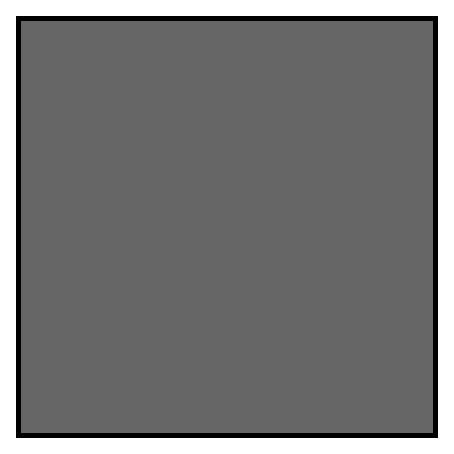
\includegraphics{example.eps}
% figure caption is below the figure
%\caption{Please write your figure caption here}
%\label{fig:1}       % Give a unique label
%\end{figure}
%
% For two-column wide figures use
%\begin{figure*}
% Use the relevant command to insert your figure file.
% For example, with the graphicx package use
%  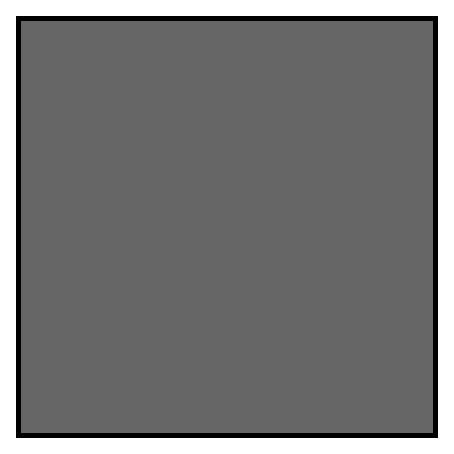
\includegraphics[width=0.75\textwidth]{example.eps}
% figure caption is below the figure
%\caption{Please write your figure caption here}
%\label{fig:2}       % Give a unique label
%\end{figure*}
%
% For tables use
%\begin{table}
% table caption is above the table
%\caption{Please write your table caption here}
%\label{tab:1}       % Give a unique label
% For LaTeX tables use
%\begin{tabular}{lll}
%\hline\noalign{\smallskip}
%first & second & third  \\
%\noalign{\smallskip}\hline\noalign{\smallskip}
%number & number & number \\
%number & number & number \\
%\noalign{\smallskip}\hline
%\end{tabular}
%\end{table}


%\begin{acknowledgements}
%If you'd like to thank anyone, place your comments here
%and remove the percent signs.
%\end{acknowledgements}


% Authors must disclose all relationships or interests that 
% could have direct or potential influence or impart bias on 
% the work: 
%
% \section*{Conflict of interest}
%
% The authors declare that they have no conflict of interest.


% BibTeX users please use one of
%\bibliographystyle{spbasic}      % basic style, author-year citations
%\bibliographystyle{spmpsci}      % mathematics and physical sciences
%\bibliographystyle{spphys}       % APS-like style for physics
%\bibliography{}   % name your BibTeX data base

% Non-BibTeX users please use
\begin{thebibliography}{}
%
% and use \bibitem to create references. Consult the Instructions
% for authors for reference list style.
%
% Format for Journal Reference
\bibitem{RefJ}

%Author, Article title, Journal, Volume, page numbers (year)


%\bibitem{wang2014role}
%Wang, Xinyu and Zhao, Liping and Wang, Ye and Sun, Jie, The role of requirements engineering practices in agile development: an empirical study, Requirements Engineering, 195-209 (2014)

\bibitem{buglione2013improving}
Buglione, Luigi and Abran, Alain, Improving the user story agile technique using the invest criteria, International Workshop on Software Measurement and International Conference on Software Process and Product Measurement IEEE, 49-53 (2013)

\bibitem{choetkiertikul2017predicting}
Choetkiertikul, Morakot and Dam, Hoa Khanh and Tran, Truyen and Ghose, Aditya, Predicting the delay of issues with due dates in software projects, Empirical Software Engineering, 22, 1223-1263 (2017)

\bibitem{abrahamsson2011predicting}
Abrahamsson, Pekka and Fronza, Ilenia and Moser, Raimund and Vlasenko, Jelena and Pedrycz, Witold, Predicting development effort from user stories, International Symposium on Empirical Software Engineering and Measurement, 400-403 (2011)

\bibitem{hearty2008predicting}
Hearty, Peter and Fenton, Norman and Marquez, David and Neil, Martin, Predicting project velocity in xp using a learning dynamic bayesian network model, IEEE Transactions on Software Engineering, 35, 124-137 (2008)

\bibitem{mahnivc2012using}
Mahni{\v{c}}, Viljan and Hovelja, Toma{\v{z}}, On using planning poker for estimating user stories, Journal of Systems and Software, 85, 2086-2095 (2012)

\bibitem{porru2016estimating}
Porru, Simone and Murgia, Alessandro and Demeyer, Serge and Marchesi, Michele and Tonelli, Roberto, Estimating story points from issue reports, International Conference on Predictive Models and Data Analytics in Software Engineering ACM, 2 (2016)

\bibitem{ziauddin2012effort}
Ziauddin, Shahid Kamal Tipu and Zia, Shahrukh, An effort estimation model for agile software development, Advances in computer science and its applications (ACSA), 2, 314-324 (2012)

\bibitem{haugen2006empirical}
Haugen, Nils Christian, An empirical study of using planning poker for user story estimation, IEEE, 9 (2006)

\bibitem{choetkiertikul2018deep}
Choetkiertikul, Morakot and Dam, Hoa Khanh and Tran, Truyen and Pham, Trang Thi Minh and Ghose, Aditya and Menzies, Tim, A deep learning model for estimating story points, IEEE Transactions on Software Engineering (2018)

\bibitem{wen2012systematic}
Wen, Jianfeng and Li, Shixian and Lin, Zhiyong and Hu, Yong and Huang, Changqin, Systematic literature review of machine learning based software development effort estimation models, Information and Software Technology, 54, 41-59 (2012)

\bibitem{femmer2017rapid}
Femmer, Henning and Fern{\'a}ndez, Daniel M{\'e}ndez and Wagner, Stefan and Eder, Sebastian, Rapid quality assurance with requirements smells, Journal of Systems and Software, 123, 190-213 (2017)

\bibitem{cleland2006detection}
Cleland-Huang, Jane and Settimi, Raffaella and Zou, Xuchang and Solc, Peter, The detection and classification of non-functional requirements with application to early aspects, IEEE International Requirements Engineering Conference, 39-48 (2006)

\bibitem{behnamghader2017large}
Behnamghader, Pooyan and Le, Duc Minh and Garcia, Joshua and Link, Daniel and Shahbazian, Arman and Medvidovic, Nenad, A large-scale study of architectural evolution in open-source software systems, Empirical Software Engineering, 22, 1146-1193 (2017)

\bibitem{shahbazian2018toward}
Shahbazian, Arman and Nam, Daye and Medvidovic, Nenad, Toward predicting architectural significance of implementation issues, International Conference on Mining Software Repositories ACM, 215-219 (2018)

\bibitem{tarawneh2017software}
Tarawneh, Mohammad Mahmoud, Software Requirements Classification using Natural Language Processing and SVD, International Journal of Computer Applications, 164 (2017)

\bibitem{dollmann2016and}
Dollmann, Markus and Geierhos, Michaela, On-and off-topic classification and semantic annotation of user-generated software requirements, Conference on Empirical Methods in Natural Language Processing, 1807-1816 (2016)

\bibitem{chen2012random}
Chen, Xi and Ishwaran, Hemant, Random forests for genomic data analysis, Genomics, 99, 323-329 (2012)

\bibitem{caruana2008empirical}
Caruana, Rich and Karampatziakis, Nikos and Yessenalina, Ainur, An empirical evaluation of supervised learning in high dimensions, international conference on Machine learning ACM, 96-103 (2008)

\bibitem{vlas2011rule}
Vlas, Radu and Robinson, William N, A rule-based natural language technique for requirements discovery and classification in open-source software development projects, Hawaii International Conference on System Sciences IEEE, 1-10 (2011)

\bibitem{pirzadeh2016reuse}
Pirzadeh, Heidar and de Santi Oliveira, Andre and Shanian, Sara, ReUse: A Recommendation System for Implementing User Stories, ICSEA, 162 (2016)

\bibitem{lai2017user}
Lai, Sen-Tarng, A User Story Quality Measurement Model for Reducing Agile Software Development Risk, International Journal of Software Engineering \& Applications, 8, 75-86 (2017)

\bibitem{desharnais2011using}
AuDesharnais, Jean-Marc and Kocaturk, Bugra and Abran, Alainthor, Using the cosmic method to evaluate the quality of the documentation of agile user stories, International Workshop on Software Measurement and International Conference on Software Process and Product Measurement, 269-272 (2011)

\bibitem{fabbrini2001linguistic}
Fabbrini, Fabrizio and Fusani, Mario and Gnesi, Stefania and Lami, Giuseppe, The linguistic approach to the natural language requirements quality: benefit of the use of an automatic tool, Annual NASA Goddard Software Engineering Workshop, 97-105 (2001)

\bibitem{bik2017reference}
Bik, Niels and Lucassen, Garm and Brinkkemper, Sjaak, A Reference Method for User Story Requirements in Agile Systems Development, IEEE International Requirements Engineering Conference Workshops, 292-298 (2017)

\bibitem{lucassen2016use}
Lucassen, Garm and Dalpiaz, Fabiano and van der Werf, Jan Martijn EM and Brinkkemper, Sjaak, The use and effectiveness of user stories in practice, International working conference on requirements engineering: Foundation for software quality, 205-222 (2016)

\bibitem{robeer2016automated}
Robeer, Marcel and Lucassen, Garm and van der Werf, Jan Martijn EM and Dalpiaz, Fabiano and Brinkkemper, Sjaak, Automated extraction of conceptual models from user stories via NLP, IEEE International Requirements Engineering Conference, 196-205 (2015)

\bibitem{lucassen2017extracting}
Lucassen, Garm and Robeer, Marcel and Dalpiaz, Fabiano and van der Werf, Jan Martijn EM and Brinkkemper, Sjaak, Extracting conceptual models from user stories with Visual Narrator, Requirements Engineering, 22, 339-358 (2017)

\bibitem{lucassen2016aqusa}
Lucassen, Garm and Dalpiaz, Fabiano and van der Werf, Jan Martijn EM and Brinkkemper, Sjaak, AQUSA: The Automatic Quality User Story Artisan for Agile Software Development, REFSQ Workshops (2016)

\bibitem{lucassen2016improving}
Lucassen, Garm and Dalpiaz, Fabiano and van der Werf, Jan Martijn EM and Brinkkemper, Sjaak, Improving agile requirements: the quality user story framework and tool, Requirements Engineering Springer, 21, 383-403 (2016)

\bibitem{lucassen2015forging}
Lucassen, Garm and Dalpiaz, Fabiano and van der Werf, Jan Martijn EM and Brinkkemper, Sjaak, Forging high-quality user stories: towards a discipline for agile requirements, IEEE international requirements engineering conference, 126-135 (2015)

\bibitem{lucassen2017improving}
Lucassen, Garm and Dalpiaz, Fabiano and van der Werf, Jan Martijn EM and Brinkkemper, Sjaak, Improving user story practice with the Grimm Method: A multiple case study in the software industry, International Working Conference on Requirements Engineering: Foundation for Software Quality Springer, 235-252 (2017)

\bibitem{wautelet2014unifying}
Wautelet, Yves and Heng, Samedi and Kolp, Manuel and Mirbel, Isabelle, Unifying and extending user story models, International Conference on Advanced Information Systems Engineering Springer, 211-225 (2014)

\bibitem{Requirements_engineering_change_sprint}
Paetsch, Frauke, Armin Eberlein, and Frank Maurer. Requirements engineering and agile software development, Twelfth IEEE International Workshops on Enabling Technologies: Infrastructure for Collaborative Enterprises, IEEE, 308-313 (2003).



\bibitem{kassab2015changing}
Kassab, Mohamad, The changing landscape of requirements engineering practices over the past decade, international workshop on empirical requirements engineering (EmpiRE), 1-8 (2015)

\bibitem{wang2014role}
Wang, Xinyu and Zhao, Liping and Wang, Ye and Sun, Jie, The role of requirements engineering practices in agile development: an empirical study, Requirements Engineering Springer, 195-209 (2014)

\bibitem{ahmed2010agile}
Ahmed, A and Ahmad, S and Ehsan, N and Mirza, E and Sarwar, SZ, Agile software development: Impact on productivity and quality, IEEE International Conference on Management of Innovation \& Technology, 287-291 (2010)

\bibitem{ortu2015jira}
Ortu, Marco and Destefanis, Giuseppe and Adams, Bram and Murgia, Alessandro and Marchesi, Michele and Tonelli, Roberto, The jira repository dataset: Understanding social aspects of software development, international conference on predictive models and data analytics in software engineering, 1 (2015)

\bibitem{chen2016xgboost}
Chen, Tianqi and Guestrin, Carlos, Xgboost: A scalable tree boosting system, ACM sigkdd international conference on knowledge discovery and data mining, 785-794 (2016)


\bibitem{le2014distributed}
Le, Quoc and Mikolov, Tomas, Distributed representations of sentences and documents, International conference on machine learning, 1188-1196 (2014)

\bibitem{dingsoyr2012decade}
Dings{\o}yr, Torgeir and Nerur, Sridhar and Balijepally, VenuGopal and Moe, Nils Brede, A decade of agile methodologies: Towards explaining agile software development, Elsevier (2012)

\bibitem{story_point_definition}
Coelho, Evita, and Anirban Basu, Effort estimation in agile software development using story points, International Journal of Applied Information Systems (IJAIS), 3.7, (2012)


\bibitem{beck2001manifesto}
Beck, Kent and Beedle, Mike and Van Bennekum, Arie and Cockburn, Alistair and Cunningham, Ward and Fowler, Martin and Grenning, James and Highsmith, Jim and Hunt, Andrew and Jeffries, Ron and others, Manifesto for agile software development (2010)

\bibitem{livermore2008factors}
Livermore, Jeffrey A, Factors that Significantly Impact the Implementation of an Agile Software Development Methodology, JSL, 3, 31-36 (2008)


\bibitem{abrahamsson2017agile}
Abrahamsson, Pekka and Salo, Outi and Ronkainen, Jussi and Warsta, Juhani, Agile software development methods: Review and analysis, arXiv preprint arXiv:1709.08439 (2017)


\bibitem{dimitrijevic2015comparative}
Dimitrijevi{\'c}, Sonja and Jovanovi{\'c}, Jelena and Deved{\v{z}}i{\'c}, Vladan, A comparative study of software tools for user story management, Information and software technology, 57, 352-368 (2015)

\bibitem{cohen2003agile}
Cohen, David and Lindvall, Mikael and Costa, Patricia, Agile software development, DACS SOAR Report, 11 (2003)


\bibitem{breiman2001random}
Breiman, Leo, Random forests, Machine learning, 45, 5-32 (2001)


\bibitem{rees2002feasible}
Rees, Michael J, Asia-Pacific Software Engineering Conference, 22-30, IEEE (2002)

\bibitem{abrahamsson2010agile}
Abrahamsson, Pekka and Oza, Nilay and Siponen, Mikko T, Agile software development, 31-59, Springer (2010)


% Format for books
\bibitem{RefB}
Author, Book title, page numbers. Publisher, place (year)









\bibitem{cohn2004user}
Cohn, Mike, User stories applied: For agile software development. Addison-Wesley Professional (2004)

\bibitem{bishop1995neural}
Bishop, Christopher M and others, Neural networks for pattern recognition, Oxford university press (1995)

\bibitem{leffingwell2010agileINVEST}
Leffingwell, Dean, Agile software requirements: lean requirements practices for teams, programs, and the enterprise, Addison-Wesley Professional (2010)

\bibitem{schwaber2002agile}
Schwaber, Ken and Beedle, Mike, Agile software development with Scrum, Prentice Hall Upper Saddle River (2002)

\bibitem{schwaber2017agile}
K. Schwaber, J. Sutherland, The scrum guide: the definitive guide to scrum:
the rules of the game. <http://www.scrum.org/scrum-guides> (2011)
(accessed 27.07.20).

\bibitem{fowler2001agile}
Fowler, Martin and Highsmith, Jim and others, 
The agile manifesto, 
Software Development, (2001). 

\end{thebibliography}

\end{document}
% end of file template.tex

